%% This is file `elsarticle-template-1-num.tex',
%%
%% Copyright 2009 Elsevier Ltd
%%
%% This file is part of the 'Elsarticle Bundle'.
%% ---------------------------------------------
%%
%% It may be distributed under the conditions of the LaTeX Project Public
%% License, either version 1.2 of this license or (at your option) any
%% later version.  The latest version of this license is in
%%    http://www.latex-project.org/lppl.txt
%% and version 1.2 or later is part of all distributions of LaTeX
%% version 1999/12/01 or later.
%%
%% The list of all files belonging to the 'Elsarticle Bundle' is
%% given in the file `manifest.txt'.
%%
%% Template article for Elsevier's document class `elsarticle'
%% with numbered style bibliographic references
%%
%% $Id: elsarticle-template-1-num.tex 149 2009-10-08 05:01:15Z rishi $
%% $URL: http://lenova.river-valley.com/svn/elsbst/trunk/elsarticle-template-1-num.tex $
%%
%% \documentclass[preprint,12pt]{elsarticle}

%% Use the option review to obtain double line spacing
\documentclass[preprint,review,12pt]{elsarticle}

%% Use the options 1p,twocolumn; 3p; 3p,twocolumn; 5p; or 5p,twocolumn
%% for a journal layout:
%% \documentclass[final,1p,times]{elsarticle}
%% \documentclass[final,1p,times,twocolumn]{elsarticle}
%% \documentclass[final,3p,times]{elsarticle}
%% \documentclass[final,3p,times,twocolumn]{elsarticle}
%% \documentclass[final,5p,times]{elsarticle}
%% \documentclass[final,5p,times,twocolumn]{elsarticle}

%% if you use PostScript figures in your article
%% use the graphics package for simple commands
%% \usepackage{graphics}
%% or use the graphicx package for more complicated commands
%% \usepackage{graphicx}
%% or use the epsfig package if you prefer to use the old commands
%% \usepackage{epsfig}

%% The amssymb package provides various useful mathematical symbols
\usepackage{amssymb}
%% The amsthm package provides extended theorem environments
%% \usepackage{amsthm}

%% The lineno packages adds line numbers. Start line numbering with
%% \begin{linenumbers}, end it with \end{linenumbers}. Or switch it on
%% for the whole article with \linenumbers after \end{frontmatter}.
\usepackage{lineno}
\usepackage{anysize}
\usepackage{latexsym}
\usepackage{pictex}
\usepackage{fancyvrb}
\usepackage{fancyhdr}
\usepackage{color}
\usepackage{graphicx}
\usepackage{subfigure}
\usepackage{rawfonts}
\usepackage{afterpage}
\usepackage[font=small,skip=0pt]{caption}
\usepackage{tabularx}
\usepackage{float}
\usepackage{color,soul}
\usepackage{makecell}
\usepackage{textcomp}
\usepackage{amsmath}
\newcommand{\RomanNumeralCaps}[1]
    {\MakeUppercase{\romannumeral #1}}
%% natbib.sty is loaded by default. However, natbib options can be
%% provided with \biboptions{...} command. Following options are
%% valid:

%%   round  -  round parentheses are used (default)
%%   square -  square brackets are used   [option]
%%   curly  -  curly braces are used      {option}
%%   angle  -  angle brackets are used    <option>
%%   semicolon  -  multiple citations separated by semi-colon
%%   colon  - same as semicolon, an earlier confusion
%%   comma  -  separated by comma
%%   numbers-  selects numerical citations
%%   super  -  numerical citations as superscripts
%%   sort   -  sorts multiple citations according to order in ref. list
%%   sort&compress   -  like sort, but also compresses numerical citations
%%   compress - compresses without sorting
%%
%% \biboptions{comma,round}

% \biboptions{}


\journal{Journal Name}

\begin{document}
\graphicspath{ {C:/Users/sbagr/Desktop/DDP_home/paper/fig_p} }

\begin{frontmatter}
%% Title, authors and addresses

%% use the tnoteref command within \title for footnotes;
%% use the tnotetext command for the associated footnote;
%% use the fnref command within \author or \address for footnotes;
%% use the fntext command for the associated footnote;
%% use the corref command within \author for corresponding author footnotes;
%% use the cortext command for the associated footnote;
%% use the ead command for the email address,
%% and the form \ead[url] for the home page:
%%
%% \title{Title\tnoteref{label1}}
%% \tnotetext[label1]{}
%% \author{Name\corref{cor1}\fnref{label2}}
%% \ead{email address}
%% \ead[url]{home page}
%% \fntext[label2]{}
%% \cortext[cor1]{}
%% \address{Address\fnref{label3}}
%% \fntext[label3]{}

\title{Investigation on the influence of tool path radius on tool wear and tool life prediction in micro-milling using neural networks}

%% use optional labels to link authors explicitly to addresses:
%% \author[label1,label2]{<author name>}
%% \address[label1]{<address>}
%% \address[label2]{<address>}

\author[1]{Sumant Bagri}
\author[2]{Ashish Manwar}
\author[3]{Alwin Varghese}
\author[4]{Soham Mujumdar}
\author[5]{Suhas S. Joshi\thanks{Address all correspondence to this author.\\Email: ssjoshi@iitb.ac.in; Fax: +91 22 2576 3842}}

\address{Department of Mechanical Engineering, Indian Institute of Technology Bombay.}

\begin{abstract}
%% Text of abstract
Since, the tool size used in micro-milling is in the micrometer range, the stability as well as the part quality strongly depend on the forces and vibrations acting on the tool. It is therefore important to monitor the micro-milling process to ensure system stability and maintain production standards and in this context monitoring and prediction system have been developed based on machine learning models. Various methods have been implemented in the past to capture the sudden failure of microtools by correlating the failure with varying process parameters. However the impact of non-linear tool paths on tool wear is not accomodated in most of these studies. The main aim of this project is to investigate the impact of semi-circular tool paths on the sudden tool failure by introducing a new process paramater called the tool path radius. An experimental setup was designed to measure sensory data such as the cutting forces, acceleration and vibration as well as the tool wear to train the neural-network models. Sensor data was segmented into individual slot data using k-means clustering and peaks-analysis algorithms and was subsequently used for statistical feature extraction. Image binarization and alignment operations were performed on the tool condition images to extract wear features such as diameter reduction as well as the wear of individual cutting edges. Wear state classification criteria were defined to categorize the tool condition into three regions of initial wear, steady-state wear and critical wear. In order to better understand the extremely complex mechanism of microtool failure, artificial neural networks as well as deep belief networks were implemented to predict the wear state as well as the remaining-useful-life of the tools. The models were trained using hyperparameter tuning techniques to improve prediction accuracy. It was found that the wear rate increased with increasing tool path radius and larger values were found to cause catastrophic failure. The major wear mechanisms were also found to vary with varying tool path radius. The neural-network models gave 93-98\% accuracy for wear state classification and RUL prediction.
\end{abstract}

\begin{keyword}
Micro end-milling \sep Tool path radius \sep Deep Neural Networks
%% keywords here, in the form: keyword \sep keyword

%% MSC codes here, in the form: \MSC code \sep code
%% or \MSC[2008] code \sep code (2000 is the default)

\end{keyword}

\end{frontmatter}

%%
%% Start line numbering here if you want
%%
%%\linenumbers

%% main text
\section{Introduction}\label{chap:intro}

Miniaturised components demand higher dimensional conformity and surface finish quality as compared to macro-sized parts. The micro-parts produced often have a very complex geometry involving multiple curvatures which require non-linear tool paths having first-order discontinuities. These will necissitate tool slowdowns and stoppages leading to unwanted fluctuations in feed rate and jerks, resulting in inconsistent machining, poor surface qualities and even tool breakage \cite{CITE1}. Tool condition monitoring (TCM) has been recognized as an important process in micro-milling operations to prevent excessive tool wear and to maintain part tolerances and surface quality \cite{CITE2}. It involves gathering multi-sensor data, such as forces, vibrations, acoustic emissions, along with capturing tool condition using optical and data-driven techniques, to generate reference models for condition and performance monitoring. \par

Data-driven methods based on machine learning algorithms as well as probabilistic models have been increasingly used for TCM in the past decade. Malekian et al. \cite{CITE2} used accelerometer, force and acoustic emission sensors to develop a sensor fusion based neuro-fuzzy model which determines the tool wear in micro-milling. Similarly, Li et al. \cite{CITE3} used force, accelerometer and AE sensors to develop a Fuzzy Neural Network (FNN) to predict the cutter flank wear in dry milling. They reported superiority of FNN, in predicting tool wear, over other multi-regression models and backpropogated neural-networks. Cho et al. \cite{CITE4} used sensory signals to train decision fusion models including support vector machine, multilayer perceptron neural network (MLP) and radial base function neural network (RGBF) for TCM. Their TCM design based on feature fusion significantly improved the accuracy of tool condition classification. Zhenhua Wu \cite{CITE5} used adaptive neuro-fuzzy inference system (ANFIS) along with support vector regression and neural network for estimating tool wear. The prediction of tool wear in milling using three popular machine learning algorithms, including ANNs, SVR, and RFs was done by Wu et al. \cite{CITE6}. Using the spindle power sensor data and ANN based regression model, Drouillet et al. \cite{CITE7} predicted remaining-useful-life (RUL) for different spindle speeds in end-milling. In a similar study for gun-drilling process, Zhang et al. \cite{CITE8} implemented a three-hidden-layer multi layer perceptron, to predict RUL. Their study provided baseline performances for many benchmark models such as gradient boosting regressor (GB), Stochastic Gradient Descent Regressor (SGD), ElasticNet (EN) to name a few, for tool condition monitoring based on RUL prediction. Another comparative study of SVR and ANN with an emerging deep neural network methodology called the deep belief networks (DBNs) was done by Chen et al \cite{CITE9}. They reported the superiority of DBNs for predicting tool wear using multi-sensor data over the other two methodologies. Addressing the issue of deploying TCM systems for industrial purposes, Li et al. \cite{CITE10} developed an audio signals based monitoring system using classification models such as CART, random forest, kNN and SVM. \par

The material removal processes during end-milling along circular and linear tool paths have been generally assumed to be similar \cite{CITE1}. The cutting tooth trajectory is epitrochoidal in circular tool paths as opposed to the circular/trochoidal tooth trajectory in linear tool paths. Thus, the material removed in each tooth pass would be different in the two tool path geometries. Consequently, the cutting force/vibration profiles produced would be different. Banerjee and Bordatchev \cite{CITE1}, investigating the impact of tool path geometry, reported that a smaller tool path radii results in lower cutting force amplitudes whereas, a larger tool path radii, equal to 50 mm, have cutting forces similar to those along the linear tool path. In a similar study, Ma et al. \cite{CITE11}, in their work on high speed milling of Ti-6Al-4V, found that the cutting forces and vibrations increase with an increase in the tool path radius. Silva and Hassui \cite{CITE12} also conducted an experimental investigation using linear, sinusoidal, triangular and sawtooth tool paths. They reported a reduction in cutting force magnitudes when using sinusoidal (45-70\%), triangular (45–70\%) and sawtooth (30–35\%) tool paths in comparison to the linear path. Shi et al. \cite{CITE13} reported that smaller tool path radii lead to greater uncut chip thickness and that adjusting feed direction can minimize cutting forces. \par

Although, a substantial amount of work has been done to develop the most optimal, data-driven, TCM system for micro-milling using sensory data and process parameters, tool path geometry remains unaccounted for. It is evident from the above review that there is a need to specifically consider the effect of circular tool paths in end-milling. The main aim of this research is to study and model the impact of circular tool paths on the tool wear and tool life in micro-end-milling using neural network based data-driven techniques. The focus here is to bridge the gap between studying the effect of tool path radius on cutting forces/vibrations and using such sensory data for a data-driven tool condition monitoring. With the goal to better understand the tool wear and to improve prediction prognostics, the wear of individual cutter edges was also separately considered. The modelling methodolgy explores the newly developing domain of deep neural networks for data-driven prognostics to predict tool condition and remaining-useful-life (RUL). We envisage that such models would be able to capture the effect of tool path radius on the wear state and life of the tool for on-line tool condition monitoring. \par

The remainder of the paper is organized into four major sections: (i) Theme and methodolgy of work, (ii) Data Acquisition and Processing, (iii) Design of neural network architecture and training and (iv) Results and discussions followed by conclusions.


\section{Experimental Details}\label{chap:exp}

\subsection{Theme of Work}\label{sec:sec31}
The theme of this work is summarized in the flow chart in Fig. \ref{fig:fig31}. \par

\begin{figure}[!h]
\begin{center}
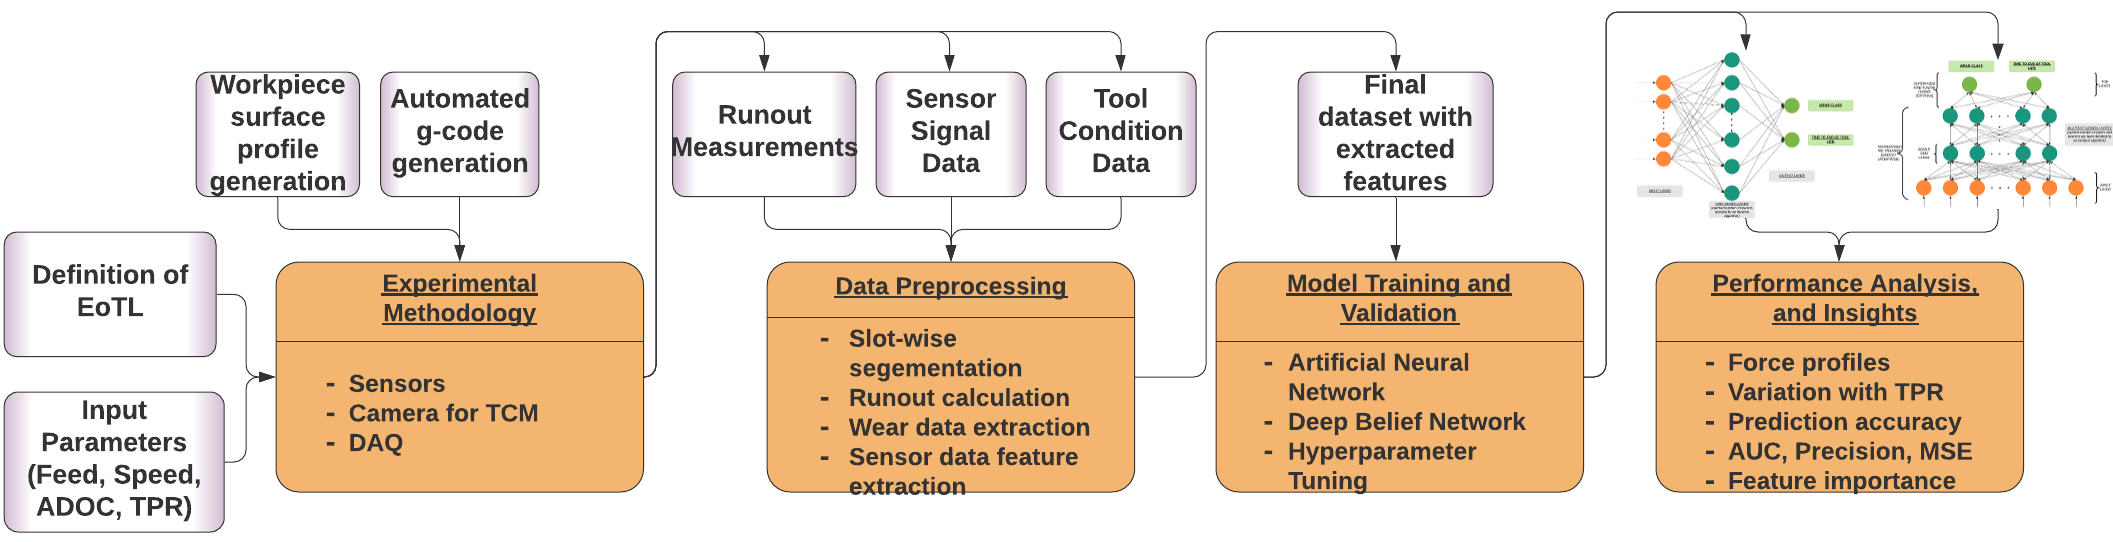
\includegraphics[width=\linewidth]{31.png}
\caption{Project work flow}\label{fig:fig31}
\end{center}
\end{figure}

 In order to understand the effect of tool-path on tool wear, curved slot milling operations were carried out with varying radius of semi-circular tool-paths as discussed in section \ref{sec:sec33} below. The experiments were carried out until the end-of-tool-life (EoTL) criteria was reached, which is defined by Eq. \ref{eq:eq31}, or until tool breakage. \par

\begin{equation}
EoTL : Diameter\,Reduction \geq 150\,\mu{m}\label{eq:eq31}
\end{equation}

The process parameters that were varied include the axial depth of cut (ADoC), feed per tooth and rotational speed of cutter. In addition, tool path radius (tpr) was also varied. The data generated from the experiments was processed to extract statistical features and output variables for classification, training, validation and testing datasets. It was then fed to two neural-network models, listed in section \ref{chap:model}, for training and evaluating prediction error on testing data using multiple metrics. \par

Two types of prediction analyses were performed; these include classification based training to predict wear category and regression-based training for prediction of RUL (remaining-useful-life). The classification based training involves training three separate models using different parameters as output labels namely: i) diameter reduction, ii) chipping area of edge 1 and iii) chipping area of edge 2 (tools with two flutes were used). The trained models were then combined to give an overall view of the tool condition. Such a combination of models to classify the wear state of each edge and the tool as a whole enables a more informed decision making process. The output from the regression based model would provide an insight into the remaining tool life. \par

\subsection{Experimental Setup}\label{sec:sec32}
The overview of the experimental setup with the signal amplifiers, DAQ console and laser vibrometer is shown the Fig. \ref{fig:fig32}(a). Fig. \ref{fig:fig32}(b) displays the workpiece setup mounted on a dynamometer along with a camera attached to the fixture, and an accelerometer placed on the spindle head. The machining center was connected to an external lubrication system to provide temperature control for high rpm spindle working conditions. The maximum speed that the spindle can reach is 140,000 RPM. The vertical linear motion in Z-direction is given to the spindle head and the X- and Y- directions are given to the table. The CNC controller is interfaced with the CNC-train software to provide programmable control over the micro-CNC machine. The zero-level in the Z-direction was setup using a camera interfaced with the DINOWARE software. \par

\begin{figure}[!h]
\begin{center}
\includegraphics[width=\linewidth]{32.png}
\caption{Complete layout of experiment (a) Overview of entire setup (b) Machining center}\label{fig:fig32}
\end{center}
\end{figure}

 One of the major goals of the experiments was to be able to capture the tool condition without removing the tool using a high resolution camera provided by Dino-Lite. In order to achieve this, a fixture was specifically designed and fabricated to house the camera. The images of the tool face were captured at a predetermined interval as is discussed in section \ref{sec:sec33}. The camera was connected to a separate system which was also used for the sensor data acquisition. \par

 The workpiece used in the experiments was a plate of grade 304 stainless steel (SS304) and had dimensions that provide 35 x 40  mm$^2$ machining area. It was mounted on the dynamometer using screws. The uncoated tungsten-carbide (WC) micro-end mills of shank diameter 3 mm and the tool diameter 500 $\mu{m}$ were used in all the experiments (see Table \ref{tab:T31} for tool specifications). The tool was fitted into a collet such that it maintains an overhang of 20 mm across all the experiments. \par

\begin{minipage}{\linewidth}
\begin{center}
\captionof{table}{Tool Specifications} \label{tab:T31}
\begin{tabular}{ c c c c c }
	\hline
	Diameter & Flute Length & Helix Angle & Overall Length & Shank Diameter \\
	\hline\hline
 	$500\,\mu$m & $1$ mm & $30\textsuperscript{o}$ & $38$ mm & $3$ mm \\
 	\hline
\end{tabular}
\end{center}
\end{minipage} \\

 The cutting forces were measured using a Kistler, compact multi-component dynamometer while the acceleration data was captured with the help of Kistler IEPE Triaxial Accelerometer. The charge signals generated from the dynamometer and the accelerometer were amplified and converted to voltage signals. In order to capture more characteristics of the system under study, vibration measurement was done using a laser doppler vibrometer (Polytec NLV-500). Its controller had a built-in signal processor, power supply unit and a laser interferometer. It is a non-intrusive method that provides signals of the tool vibration velocity.\par

\subsection{Design of Experiments}\label{sec:sec33}
The process parameters and their corresponding levels are listed in Table \ref{tab:T33}. \par

\begin{minipage}{\linewidth}
\begin{center}
\captionof{table}{Experimental process parameters and levels} \label{tab:T33}
\begin{tabular}{ c | c c c}
	\hline
	Parameters & Level 1 & Level 2 & Level 3 \\
	\hline\hline
 	Feed ($\mu${m}/tooth) & $4$ & $6$ & $8$ \\
 	\hline
 	Spindle speed (RPM) & $40000$ & $50000$ & $60000$ \\
 	\hline
  DOC ($\mu${m}) & $50$ & $80$ & $110$ \\
  \hline
  Tool Path Radius ($\mu${m}) & $250$ & $500$ & $750$ \\
  \hline
\end{tabular}
\end{center}
\end{minipage} \\

 In order to best accomodate for the variability in machining parameters, a design of experiment involving a $3$-level, orthogonal array was used. Eight experiments were performed till the end of tool life using the parametric conditions given in Table \ref{tab:T35}. \par

\begin{minipage}{\linewidth}
  \captionof{table}{Final experimental process parameters} \label{tab:T35}
  \centering
    \begin{tabular}{ c | c c c c c }
    	\hline
    	\makecell{Experiment \\ No.} & \makecell{Tool Id} & \makecell{Feed Rate \\ (mm/s)} & RPM & \makecell{Depth \\ of cut} & \makecell{Tool path \\ radius} \\
    	\hline\hline
      $1$ & $T79$ & $16$	& $60000$ &	$80$ & $250$ \\
      \hline
      $2$ & $T80$ & $10$	& $50000$ &	$80$ & $250$ \\
      \hline
     	$3$ &	$T81$ & $5.33$	& $40000$ &	$50$ & $250$ \\
     	\hline
      $4$ & $T82$ & $10.67$	& $40000$ &	$110$ & $500$ \\
      \hline
      $5$ & $T83$ & $12$	& $60000$ &	$50$ & $500$ \\
      \hline
     	$6$ &	$T84$ & $6.67$	& $50000$ &	$80$ & $500$ \\
     	\hline
      $7$ & $T85$ & $8$	& $60000$ &	$110$ & $750$ \\
      \hline
      $8$ & $T86$ & $13.33$	& $50000$ &	$50$ & $750$ \\
      \hline

    \end{tabular}
\end{minipage} \\\\


 One of the key features of the experiments was generation of semi-cicular tool paths with varying radius. A photograph of a typical workpiece after machining is shown in Fig. \ref{fig:fig34}(a) and the tool path geometry for each slot is shown in Fig. \ref{fig:fig34}(b). A circular tool path constantly changes the feed direction in a sinusoidal manner and is therefore expected to affect tool wear progression differently than a straight line path. The photographs of the worn tools were taken at smaller or larger intervals depending upon whether the previous image of the tool indicated a severe or insignificant degradation, respectively. \par

\begin{figure}[!h]
\begin{center}
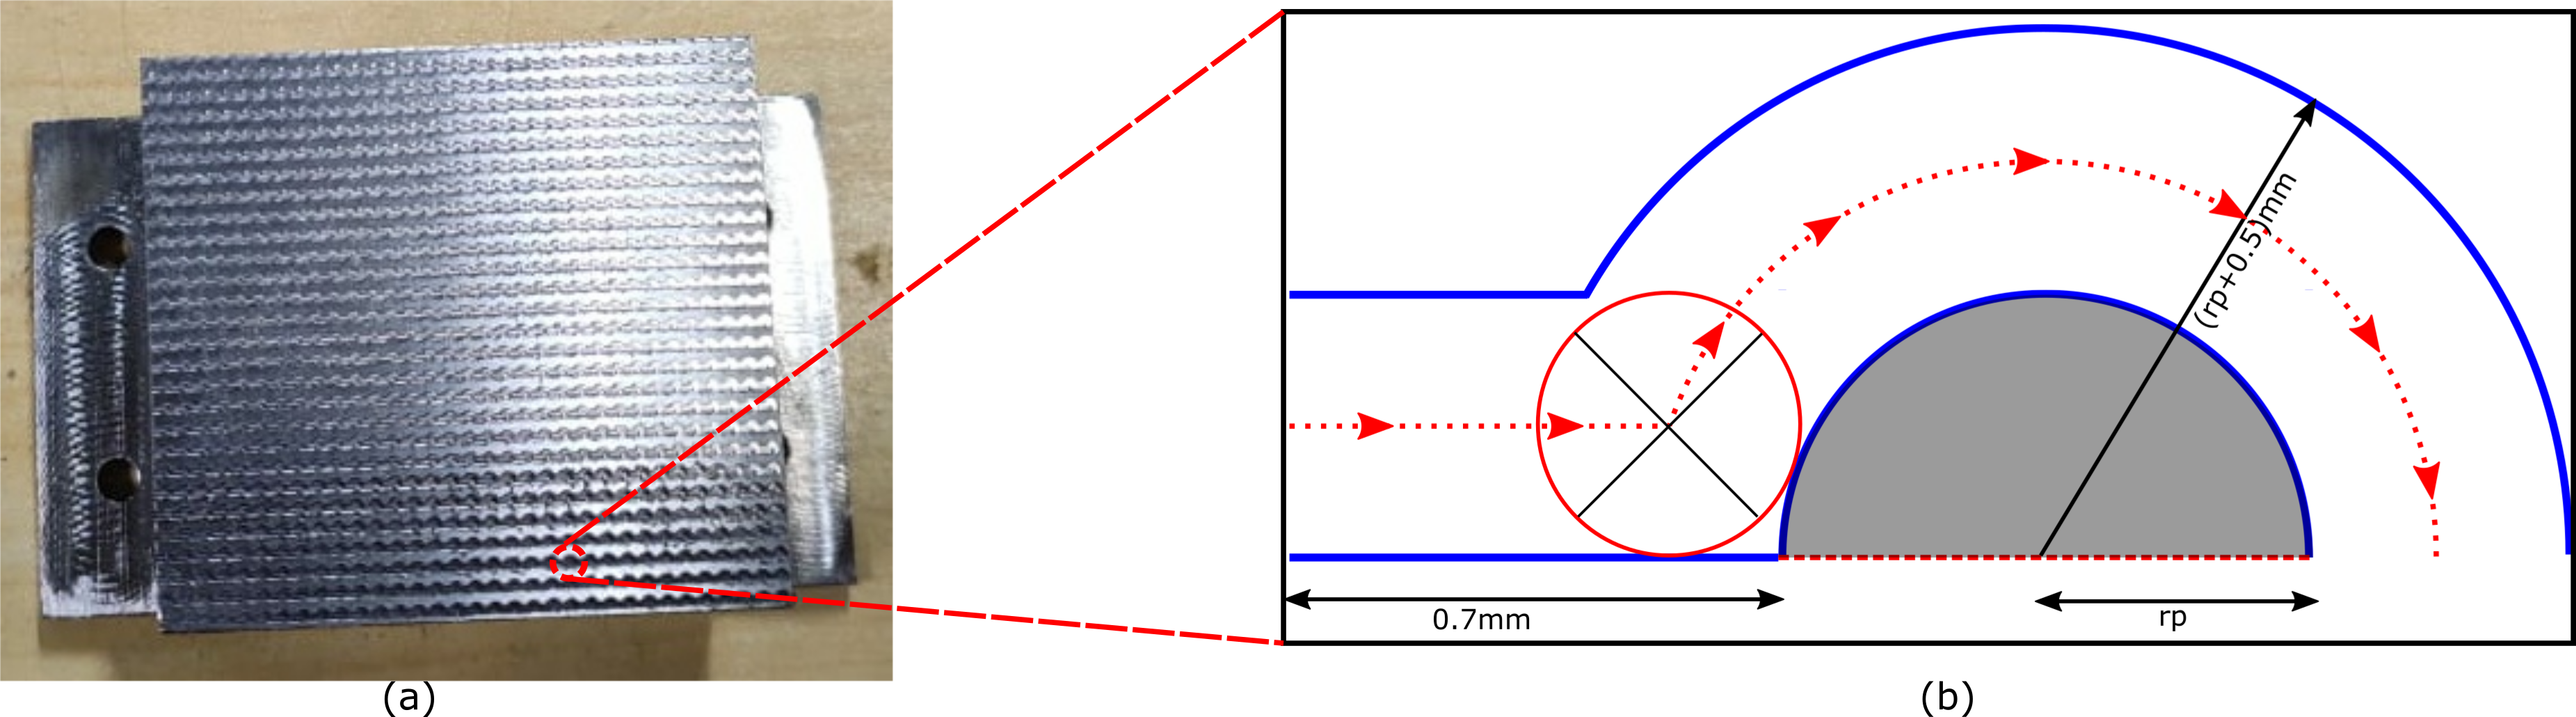
\includegraphics[width=\linewidth]{34.png}
\caption{Tool path design (a) Workpiece after machining (b) Tool path geometry}\label{fig:fig34}
\end{center}
\end{figure}

\subsection{Experimental Procedure}\label{sec:sec34}
 The main components of the experimental procedure are described in the flow chart displayed in Fig \ref{fig:fig35}. \par

\begin{figure}[!h]
\begin{center}
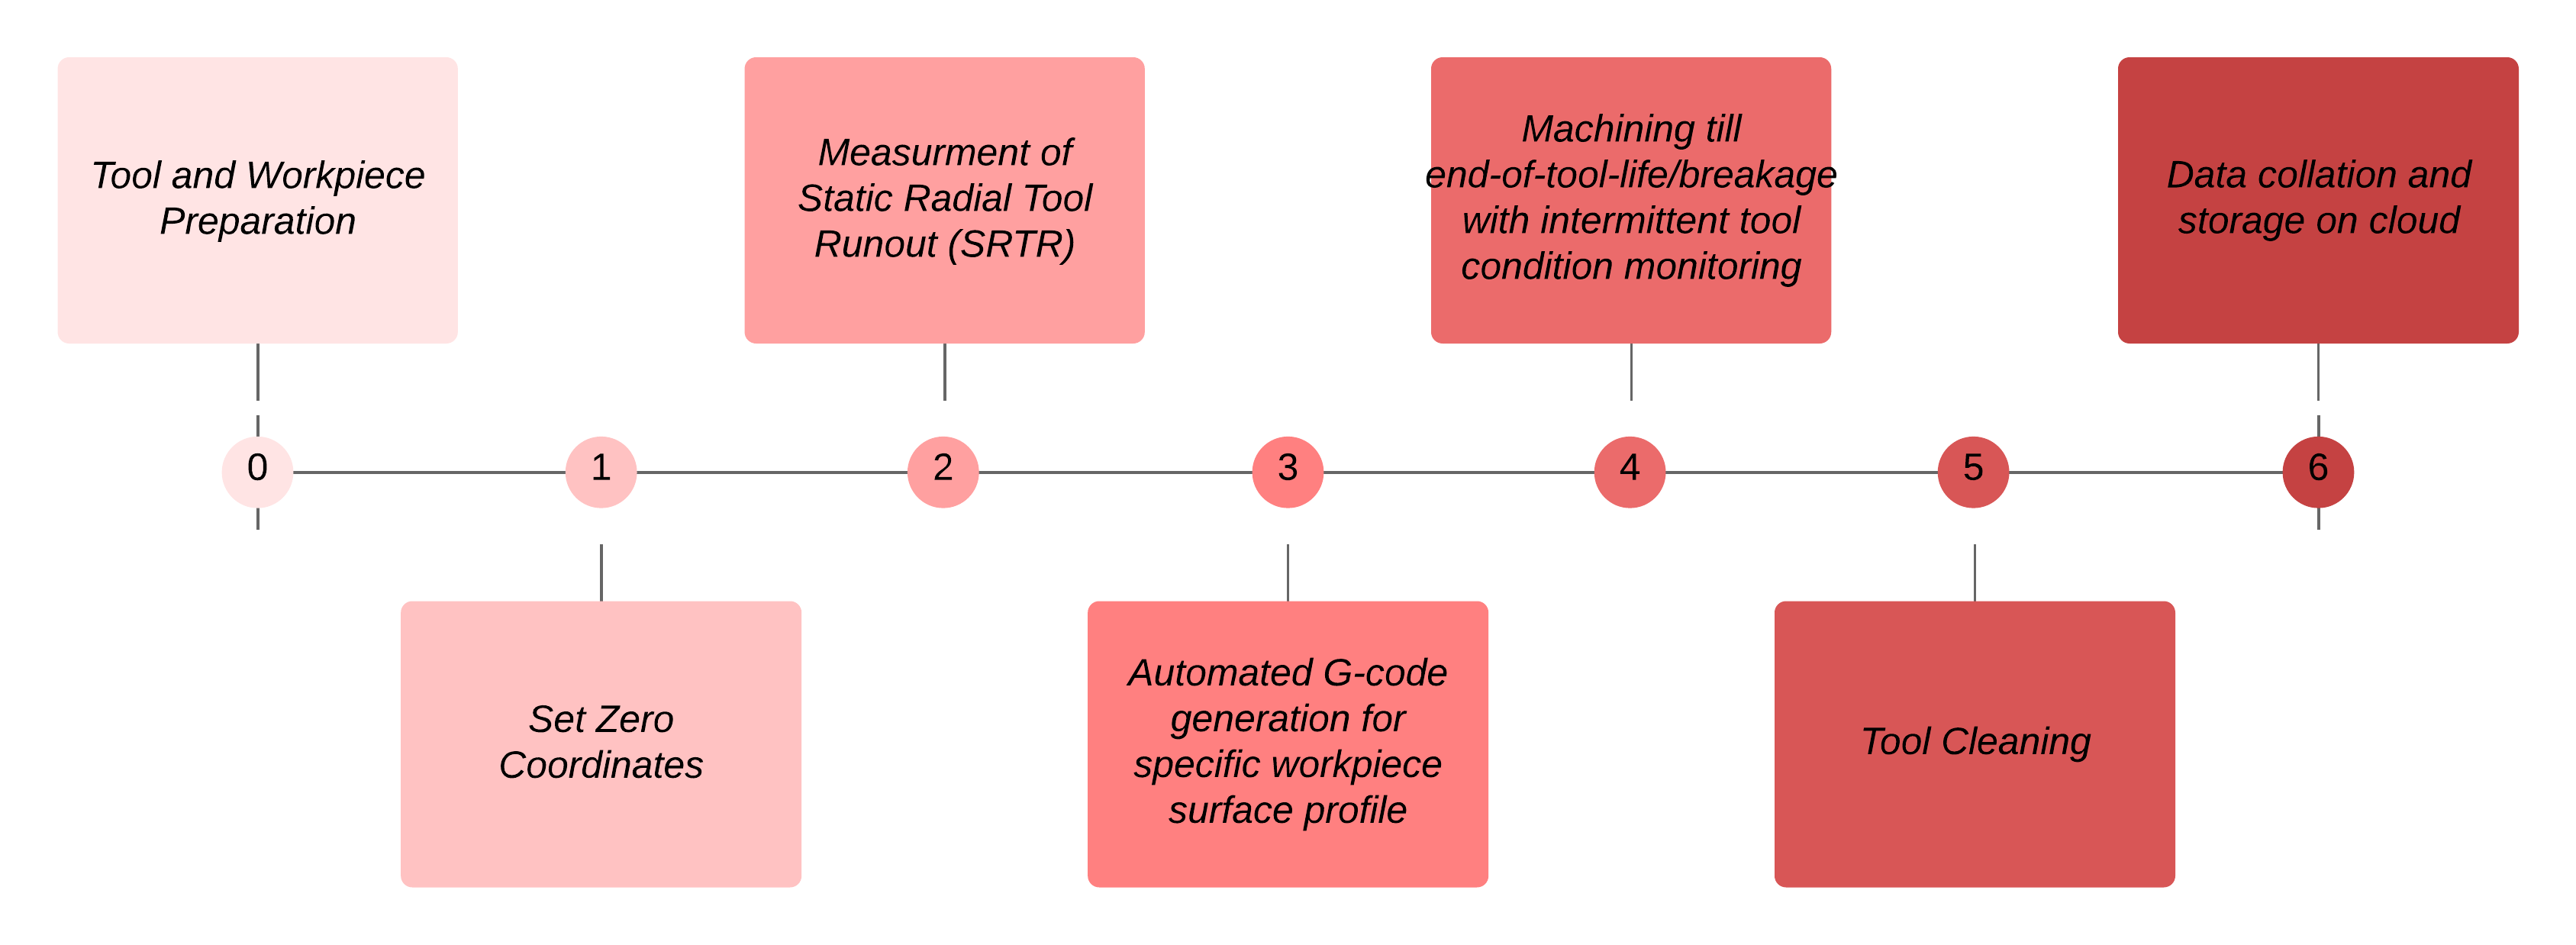
\includegraphics[width=\linewidth]{35.png}
\caption{Flow for experimental protocol}\label{fig:fig35}
\end{center}
\end{figure}

\subsubsection{Tool and workpiece preparation}
One of the major goals was to reduce the exacerbation of tool wear due to varying static runout caused by repeated removal of the tool. By keeping the tool in-situ throughout each experiment ensured consistent static tool-runout which was measured before starting the experiments. The zero coordinates of the micro-CNC machine were then set using a separate, low resolution camera. The initial image of the tool was then captured and saved while maintaining relative position of the two flutes with the help of a marking. This helped in tracking the wear of each flute while maintaining consistency. Subsequently the static radial tool runout of the tool was captured to be given as an input parameter to the machine learning model. This was achieved by taking tool images rotated at an interval of $30$\textdegree. The static radial runout can be obtained by measuring the distance between the centers of a pair of images phase-shifted by $180$\textdegree. \par

\iffalse
In order to address the issue of workpiece surface perpendicularity after mounting on the dynamometer, the surface profile was generated (Fig. \ref{fig:fig36}(a)) by touching the tool at various points on the workpiece surface and measuring the z-coordinate. The 2D linear regression fit for surface profile generation in shown in Fig. \ref{fig:fig36}(b). The z-values for slotting were then adjusted accordingly to maintain a constant depth-of-cut.

\begin{figure}[!h]
  \begin{center}
    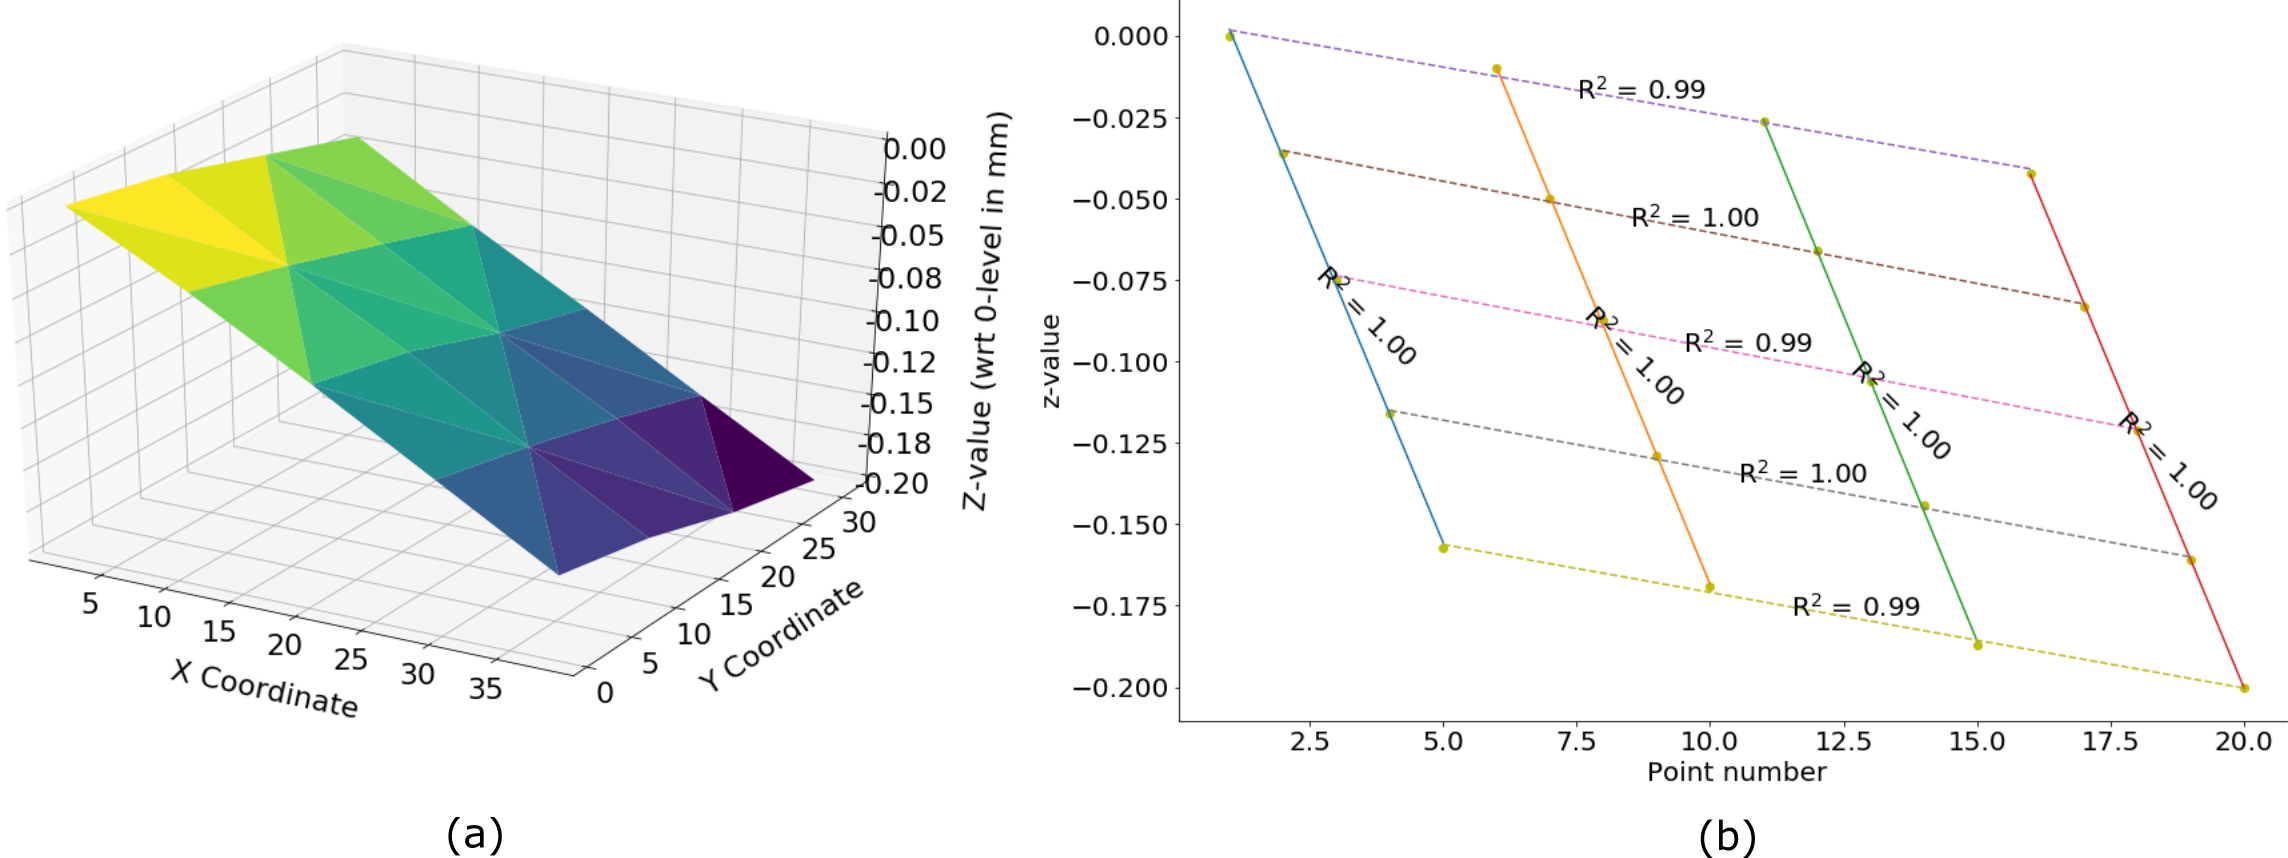
\includegraphics[width=\linewidth]{36.png}
    \caption{Workpiece surface profile: (a) 3D surface plot (b) linearity of surface profile variation}\label{fig:fig36}
  \end{center}
\end{figure}
\fi

\subsubsection{G-code Generation for Slot Milling}
Since the machining strategy involved using dynamic batch sizes for number of slots machined, large number of G-code files were obtained by automating the process of G-code generation using a Python script. Fig. \ref{fig:fig38} shows the entire flow for generation of G-codes which is described as follows. The microtool was used as a coordinate measuring tool and was touched at different locations on the workpiece surface. The z-coordinates at these locations were recorded and passed to a multiple linear regression model. This model would be fit based on the input z-coordinates and subsequently be used as a mathematical representation of the workpiece surface. This representation along with the feed rate and tool path radius was passed to the python script which then generated necessary G-codes to machine the entire workpiece with variable slot numbers (batch sizes of 5-slots, 15-slots and 30-slots). The slots were then machined until the end-of-tool-life criteria was reached as described in Eq. \ref{eq:eq31} or till tool breakage. \par

\begin{figure}[!h]
  \begin{center}
    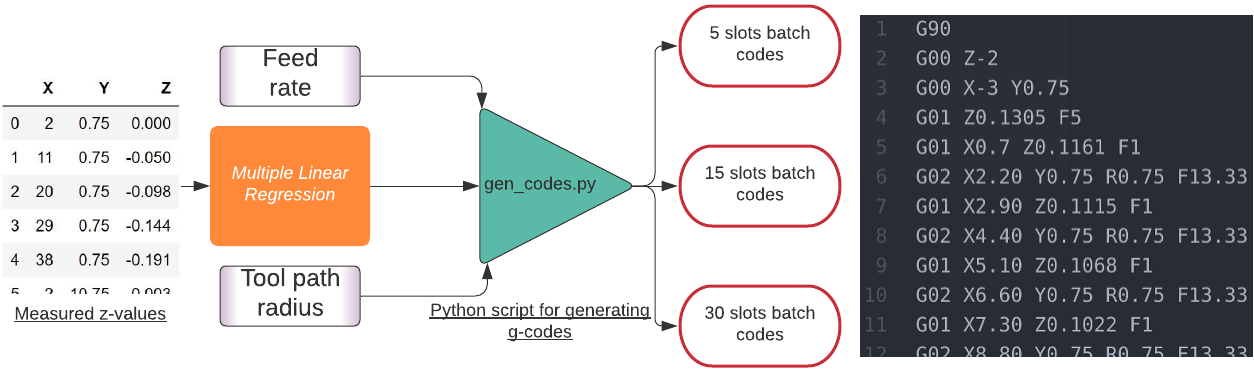
\includegraphics[width=\linewidth]{38.png}
    \caption{Automated G-code generation}\label{fig:fig38}
  \end{center}
\end{figure}

\subsubsection{Post-slot-milling}
After machining each batch of slots, tools were cleaned and their condition was recorded using a high-resolution camera. The orientation of the tool was adjusted using a marker on the tool, to maintain the relative flute position while taking the images. The sensor data stream was also stopped at this point and stored in a separate file in the DAQ system. After each experiment is completed, the entire dataset was stored on the cloud for ease of accessibility.\par



\section{Data Processing}\label{chap:data_pro}
After the data acquisition, preprocessing techniques were employed; see Fig. \ref{fig:fig39} for the data processing flow.

\begin{figure}[H]
\begin{center}
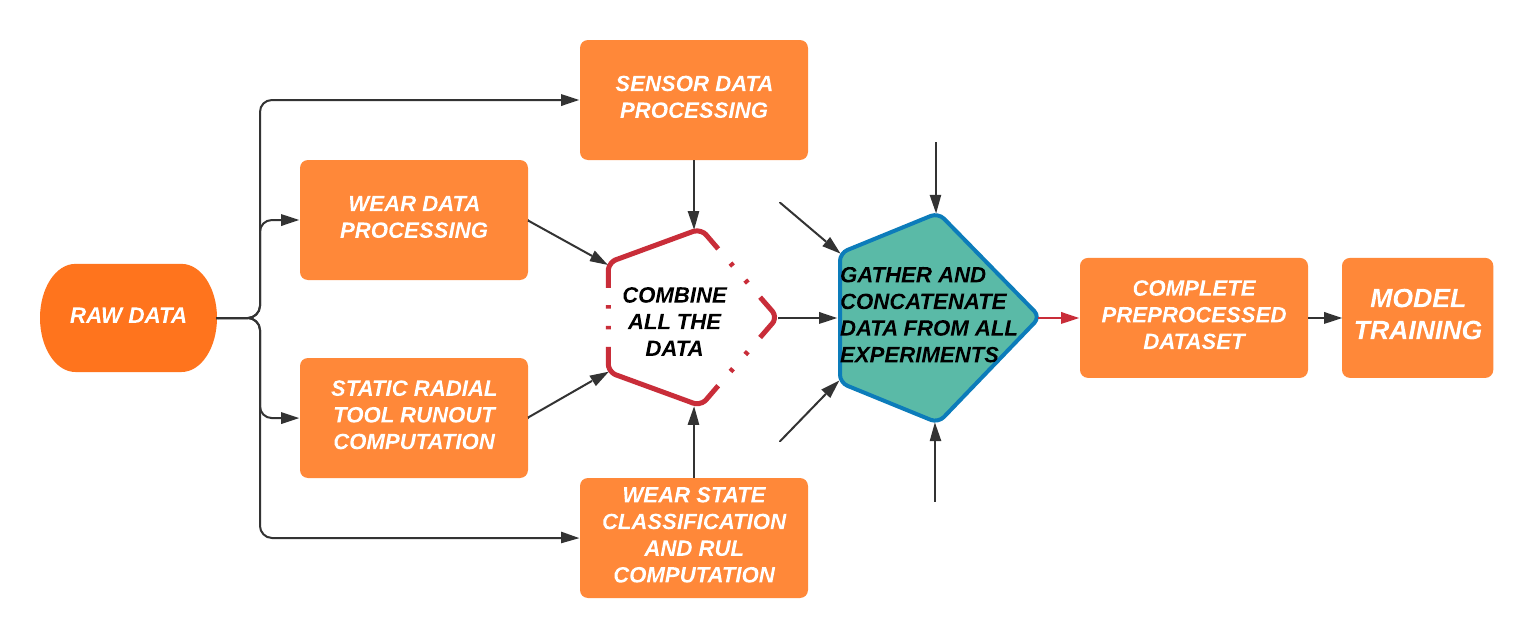
\includegraphics[width=\linewidth]{39.png}
\caption{Data preprocessing flow}\label{fig:fig39}
\end{center}
\end{figure}

\subsection{Sensor Data Preprocessing}\label{sec:sec41}
 The data files for all slot batches were imported into the working environment recursively, one at a time. The columns in the raw imported dataset were as listed: time, forces (x-, y-, z-directions), acceleration (x-, y-, z-directions) and vibration velocity. Each of the sensor data columns were multiplied by corresponding multiplication factors. Subsequently, the machining and non-machining data-points were identified using K-means clustering analysis with 10 clusters. K-means clustering is an unsupervised machine learning technique for clustering the dataset into k different groups. The red circles in Fig. \ref{fig:fig310} are the centroids of the 10 different clusters which indicate a further grouping of the data into two categories as shown. Inorder to further improve identification of start and endpoints of the machining and non-machining data, a peaks-analysis algorithm was implemented. This algorithm analyzes the variation in peak amplitudes of the data to detect cluster boundaries with a higher precision. \par

\begin{figure}[!h]
\begin{center}
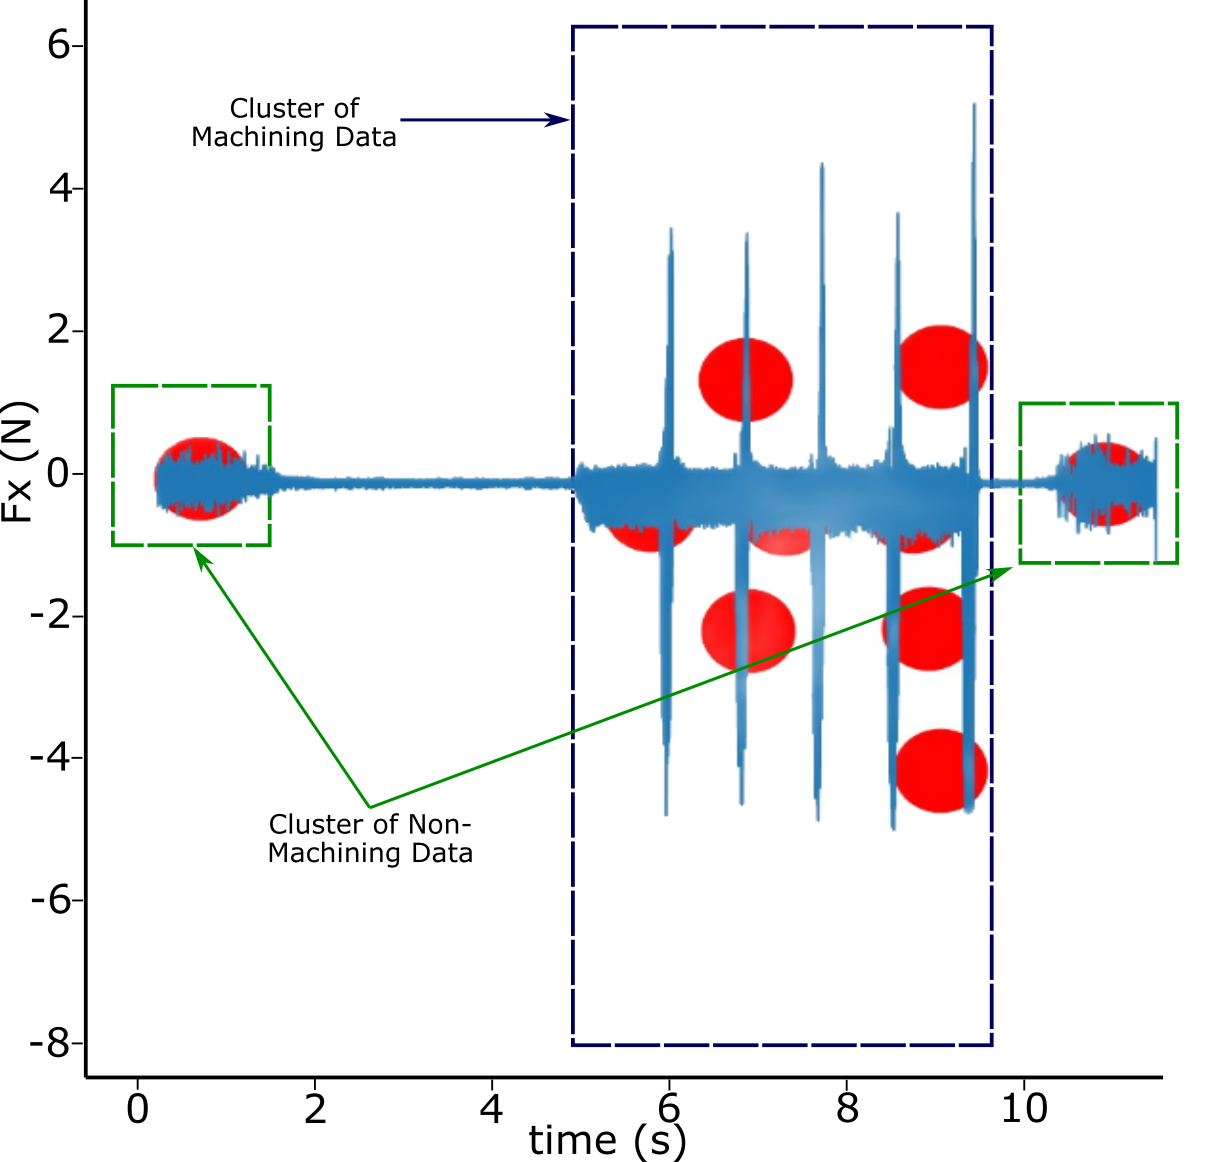
\includegraphics[width=0.7\linewidth]{310.png}
\caption{Machining and non-machining clustering}\label{fig:fig310}
\end{center}
\end{figure}

Using the peaks-analysis algorithm, the combined, semi-circular slot data was obtained from the machining data as shown in Fig. \ref{fig:fig312}(a). This was then subjected to further segmetation into individual slot data, see Fig. \ref{fig:fig312}(b). The fine-tuning of the individual slot data involved detecting and removing noise and trimming the slot data to a higher precision. The final slot-wise segmented data transformation is displayed in Fig. \ref{fig:fig312}(c). Subsequently, each slot data was further segmented into 4 parts for statistical feature extraction as described in Table \ref{tab:T36}. At this point, the various process paramters: ADOC (axial depth-of-cut), feed, spindle speed and tpr (tool path radius), are also concatenated to the dataset. \par

 \begin{figure}[!h]
   \begin{center}
     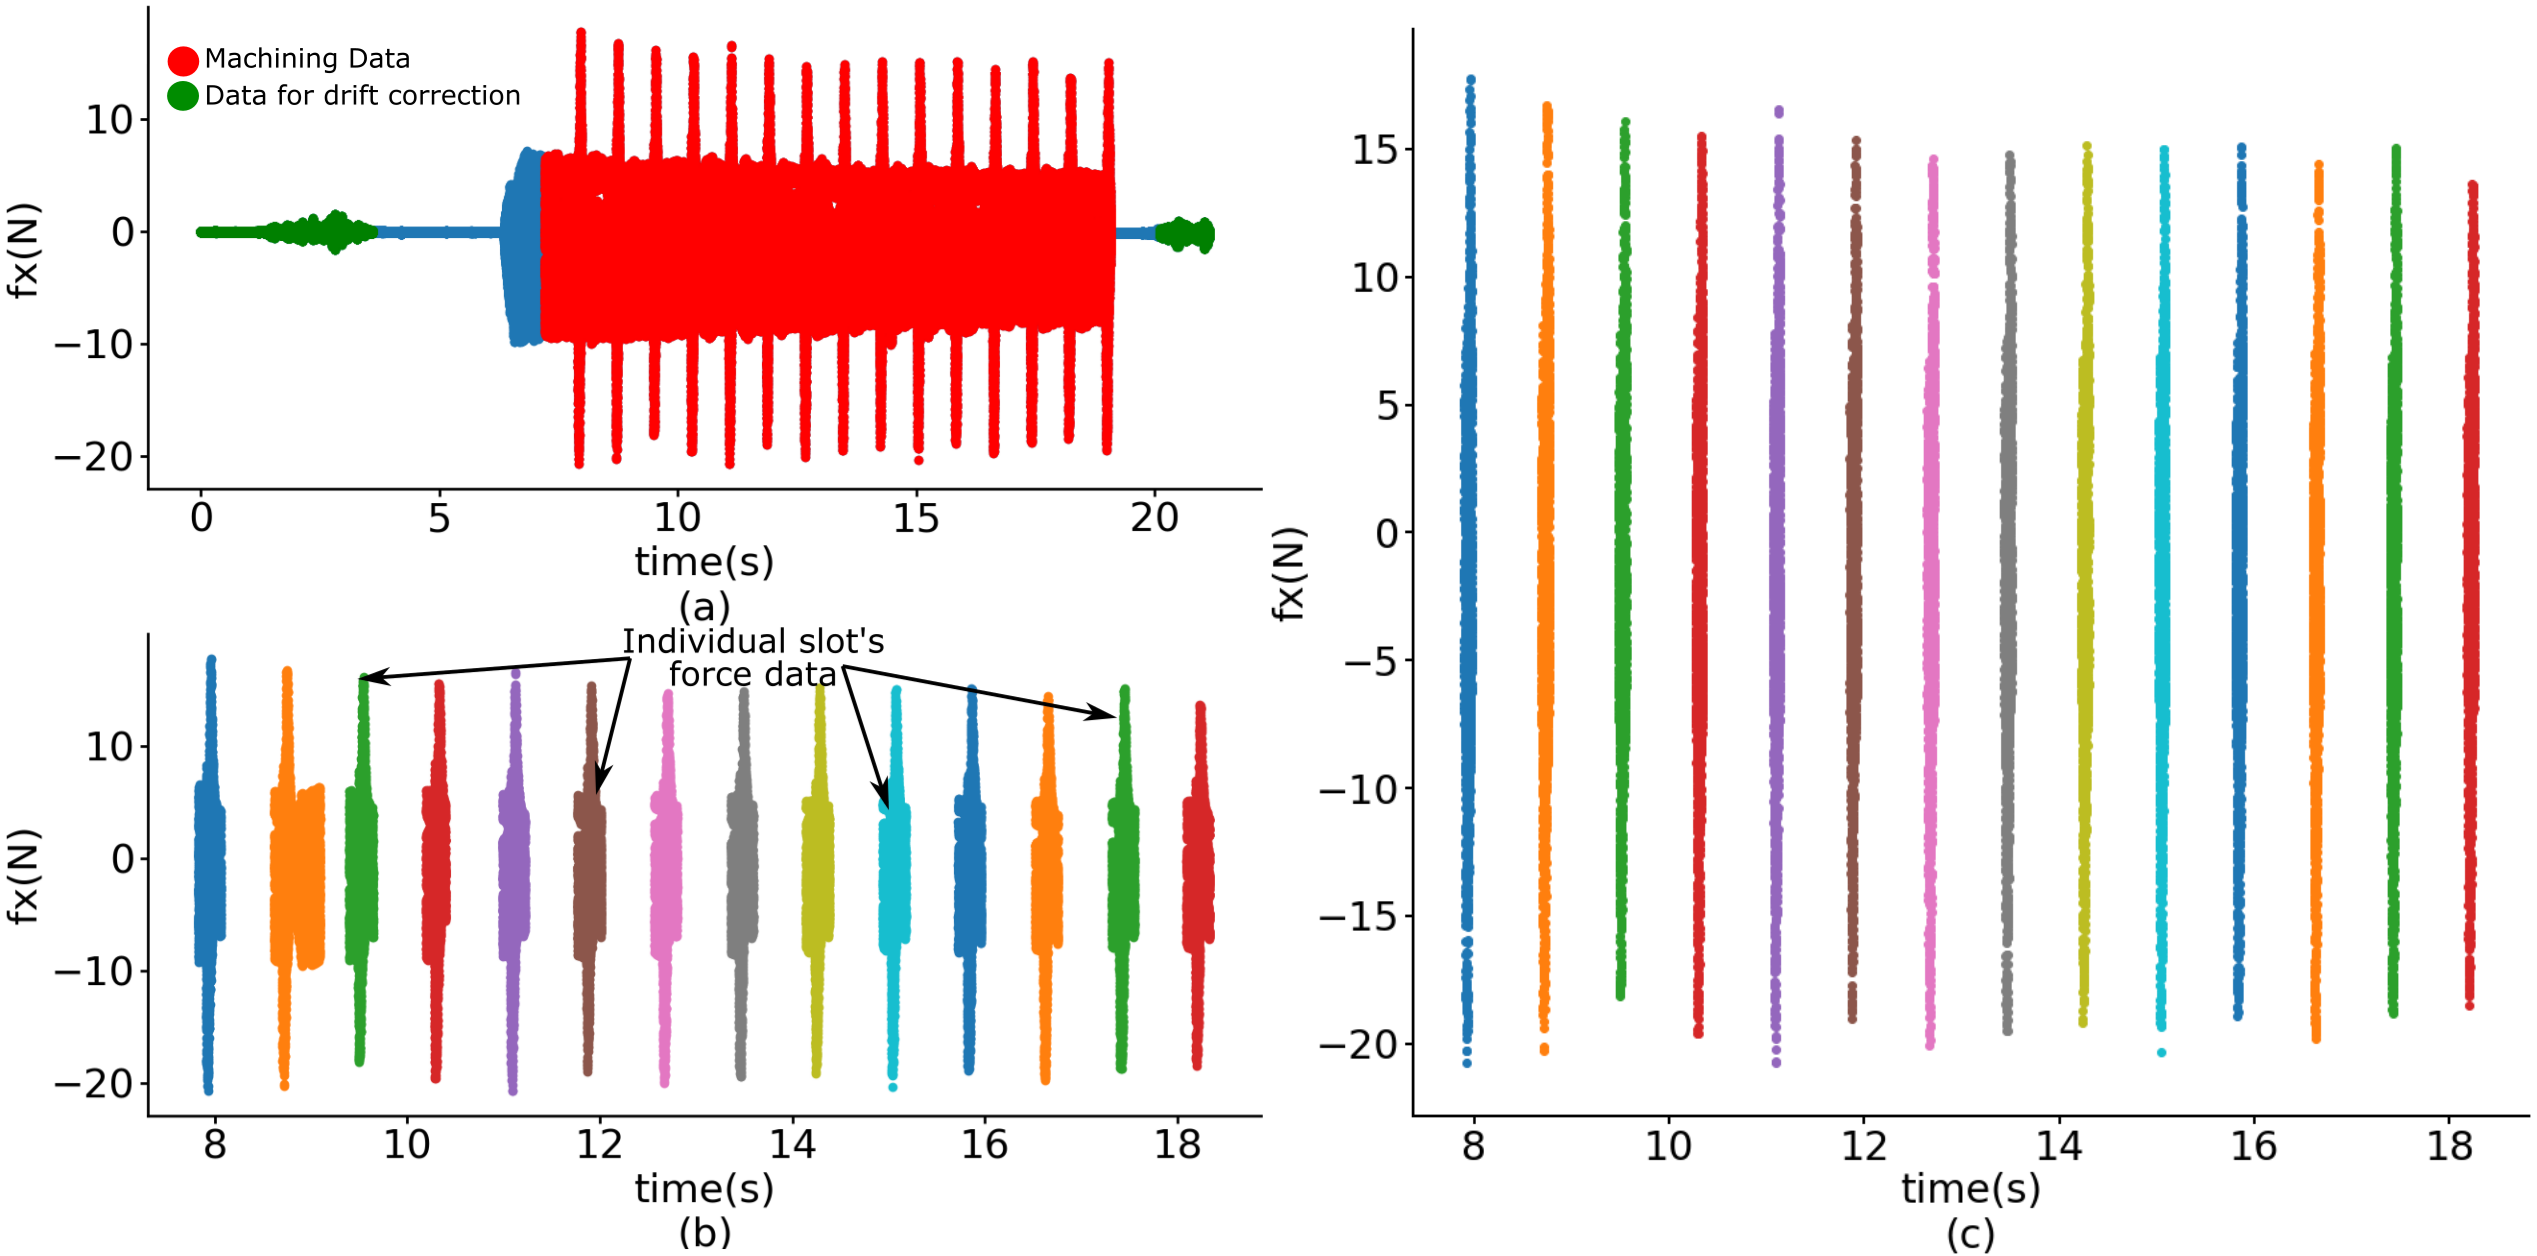
\includegraphics[width=\linewidth]{312.png}
     \caption{Slot segmentation: (a) Initial segmentation (b) Slot data detection (b) Fine-tuning detected slot data}\label{fig:fig312}
   \end{center}
 \end{figure}

\begin{minipage}{\linewidth}
  \captionof{table}{Feature extraction for sensor data} \label{tab:T36}
  \centering
    \begin{tabular}{ c c c c c c }
    	\hline
    	Fx & Fy & Fz & Vx & Vy & Vz \\
    	\hline\hline
     	Mean & Mean & Mean & Mean & Mean & Mean \\
     	\hline
     	RMS & RMS & RMS & RMS & RMS & RMS \\
     	\hline
      Std.Dev & Std.Dev & Std.Dev & Std.Dev & Std.Dev & Std.Dev \\
      \hline
      Max & Max & Max & Max & Max & Max \\
      \hline
      Min & Min & Min & Min & Min & Min \\
      \hline
      Kurtosis & Kurtosis & Kurtosis & Kurtosis & Kurtosis & Kurtosis \\
      \hline
      Skewness & Skewness & Skewness & Skewness & Skewness & Skewness \\
      \hline
      Rate & Rate & Rate & Rate & Rate & Rate \\
      \hline
    \end{tabular}
\end{minipage} \\\\

\subsection{Wear Data preprocessing}\label{sec:sec42}
All the steps involved in the wear data preprocessing are shown in Fig. \ref{fig:fig325}. \par

\begin{figure}[!h]
\begin{center}
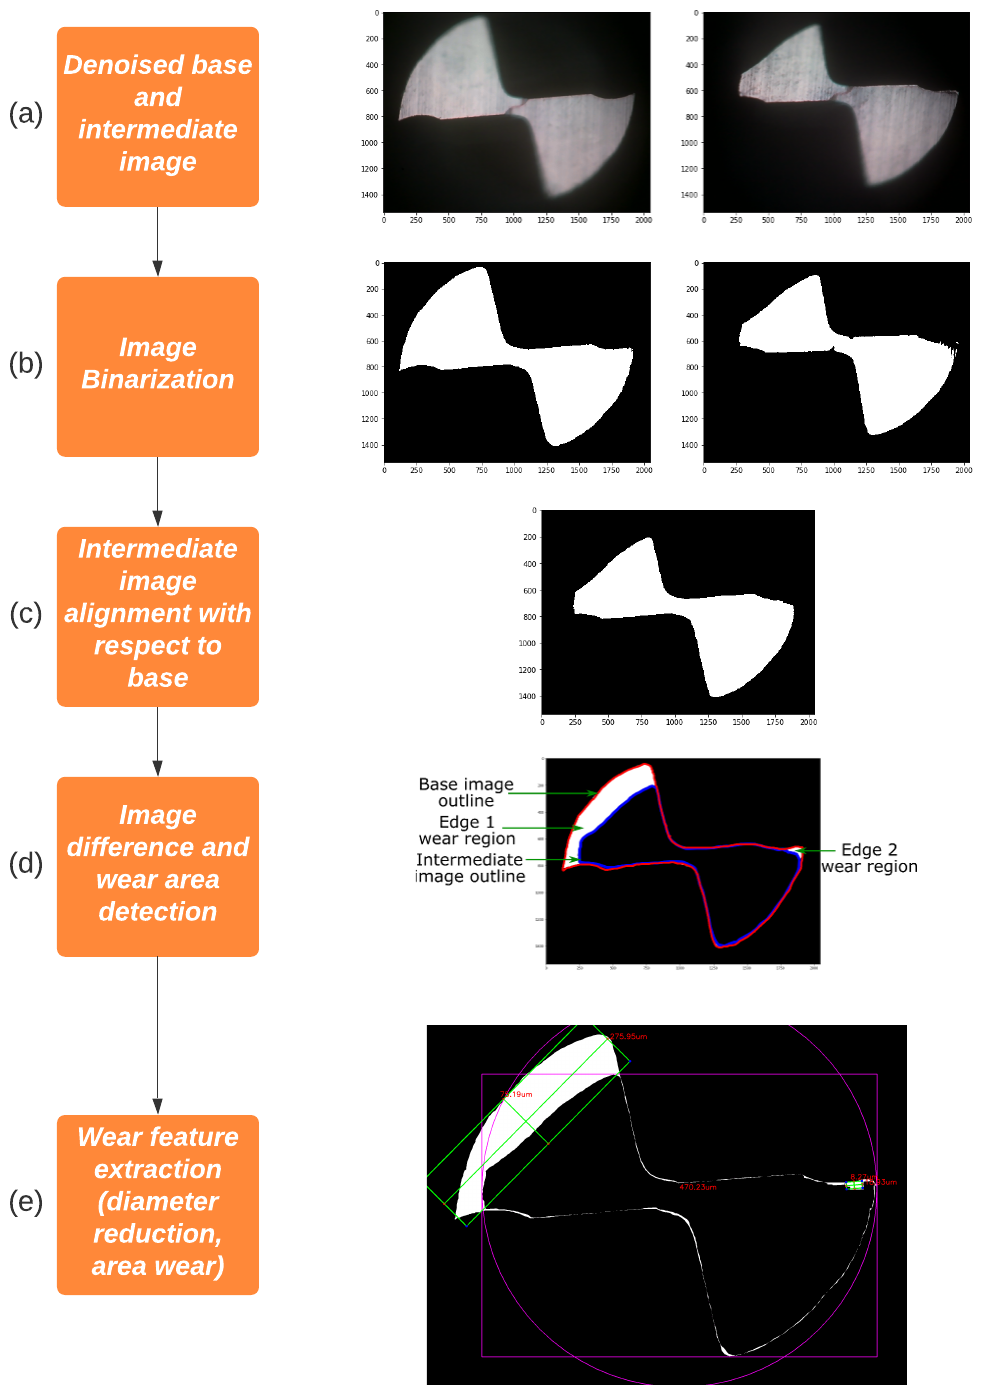
\includegraphics[width=0.7\linewidth]{325.png}
\caption{Wear data processing flow (a-e, steps involved)}\label{fig:fig325}
\end{center}
\end{figure}

The original, denoised, pre-machining tool image (Fig. \ref{fig:fig325}(a)) was captured along with an intermediate, denoised tool image. The colour images were then converted into binary format (pixels values either 0 or 255) which are shown in Fig. \ref{fig:fig325}(b). In order to remove the unwanted features, the binarized images were subjected to a few iterations of dilation-erosion. The dilation procedure adds pixels to the boundaries of objects in an image, while erosion removes pixels on object boundaries. Fig. \ref{fig:fig325}(c) shows an intermediate image aligned with respect to the base image. This was done to obtain an accurate measurement of the wear regions. Finally, Fig. \ref{fig:fig325}(d) shows the image obtained after taking a difference between the base and the intermediate image. The representative tool image in Fig. \ref{fig:fig325}(d) shows the boundaries of the base and intermediate images along with the detected wear region on each cutting edge. This image was used to calculate the contours and subsequently the bounding boxes as shown in Fig. \ref{fig:fig325}(e). The measurements of the extracted wear features were then made in pixels and subsequently converted to micrometer units using a parameter called pixels-per-metric (ppm). It was defined using the tool diameter value in micrometers (500 $\mu{m}$) and the tool diameter measured in pixels from the base image. \par

A sample dataset of the extracted wear features is shown in Table. \ref{tab:T37}. $orE1$ and $orE2$ represent the orientation of the measured wear (1 is chipping and 2 is flank wear) for each cutting edge. \emph{wear1Ei} (in $\mu{m}$) represents the length, whereas \emph{wear2Ei} (in $\mu{m}$), the breadth, of the rectangular wear area bounding box for each cutting edge \emph{i} (equal to 1 for left edge and 2 for right edge). \emph{wearAEi} (in $\mu{m}^2$) is wear of chipped area for each edge. \par

\begin{minipage}{\linewidth}
  \captionof{table}{Snapshot of wear data} \label{tab:T37}
  \centering
  \resizebox{\textwidth}{!}{
    \begin{tabular}{ c|c|c|c|c|c|c|c|c|c }
      \hline
      $slot$ & $orE1$ & $orE2$ & $dRed$  & $wearAE1$ & $wear1E1$ & $wear2E1$ & $wearAE2$ & $wear2E1$ & $wear2E2$ \\ \hline\hline
      $5   $ & $1$ & $1$ & $34.7 $ & $330.25 $ & $61.9   $ & $8.53   $ & $2169.27$ & $174.58 $ & $54.14$   \\ \hline
      $10  $ & $1$ & $1$ & $39   $ & $424.61 $ & $66.18  $ & $10.71  $ & $2148.64$ & $167.53 $ & $26.19$   \\ \hline
      $15  $ & $1$ & $1$ & $67.31$ & $676.64 $ & $73.94  $ & $16.42  $ & $9849.77$ & $266.93 $ & $62$      \\ \hline
      $20  $ & $1$ & $1$ & $66.86$ & $433.2  $ & $50.67  $ & $13.94  $ & $9760.28$ & $266.67 $ & $61.27$   \\ \hline
      $25  $ & $1$ & $1$ & $68.92$ & $574.36 $ & $70.37  $ & $15.83  $ & $9920.73$ & $266.88 $ & $62.29$   \\ \hline
    \end{tabular}
 }
\end{minipage} \\\\

\subsection{Computing the Static Radial Tool Runout}\label{sec:sec43}
 The pre-machining images captured after installing on the machining center, at a rotation interval of $30$\textdegree, were used to compute the static radial runout of the tool. Fig. \ref{fig:fig320}(a) shows the binarized image obtained from the colour image which was used for edge detection (Fig. \ref{fig:fig320}(b)). The detected edges were then used for obtaining the contours and the bounding box (Fig. \ref{fig:fig320}(c)). The images thus obtained were grouped in pairs with a phase difference of $180$\textdegree. The distance between centers of such pairs, divided by two, gives the radial runout value (Fig. \ref{fig:fig320}(d)). \par

\begin{figure}[!h]
\begin{center}
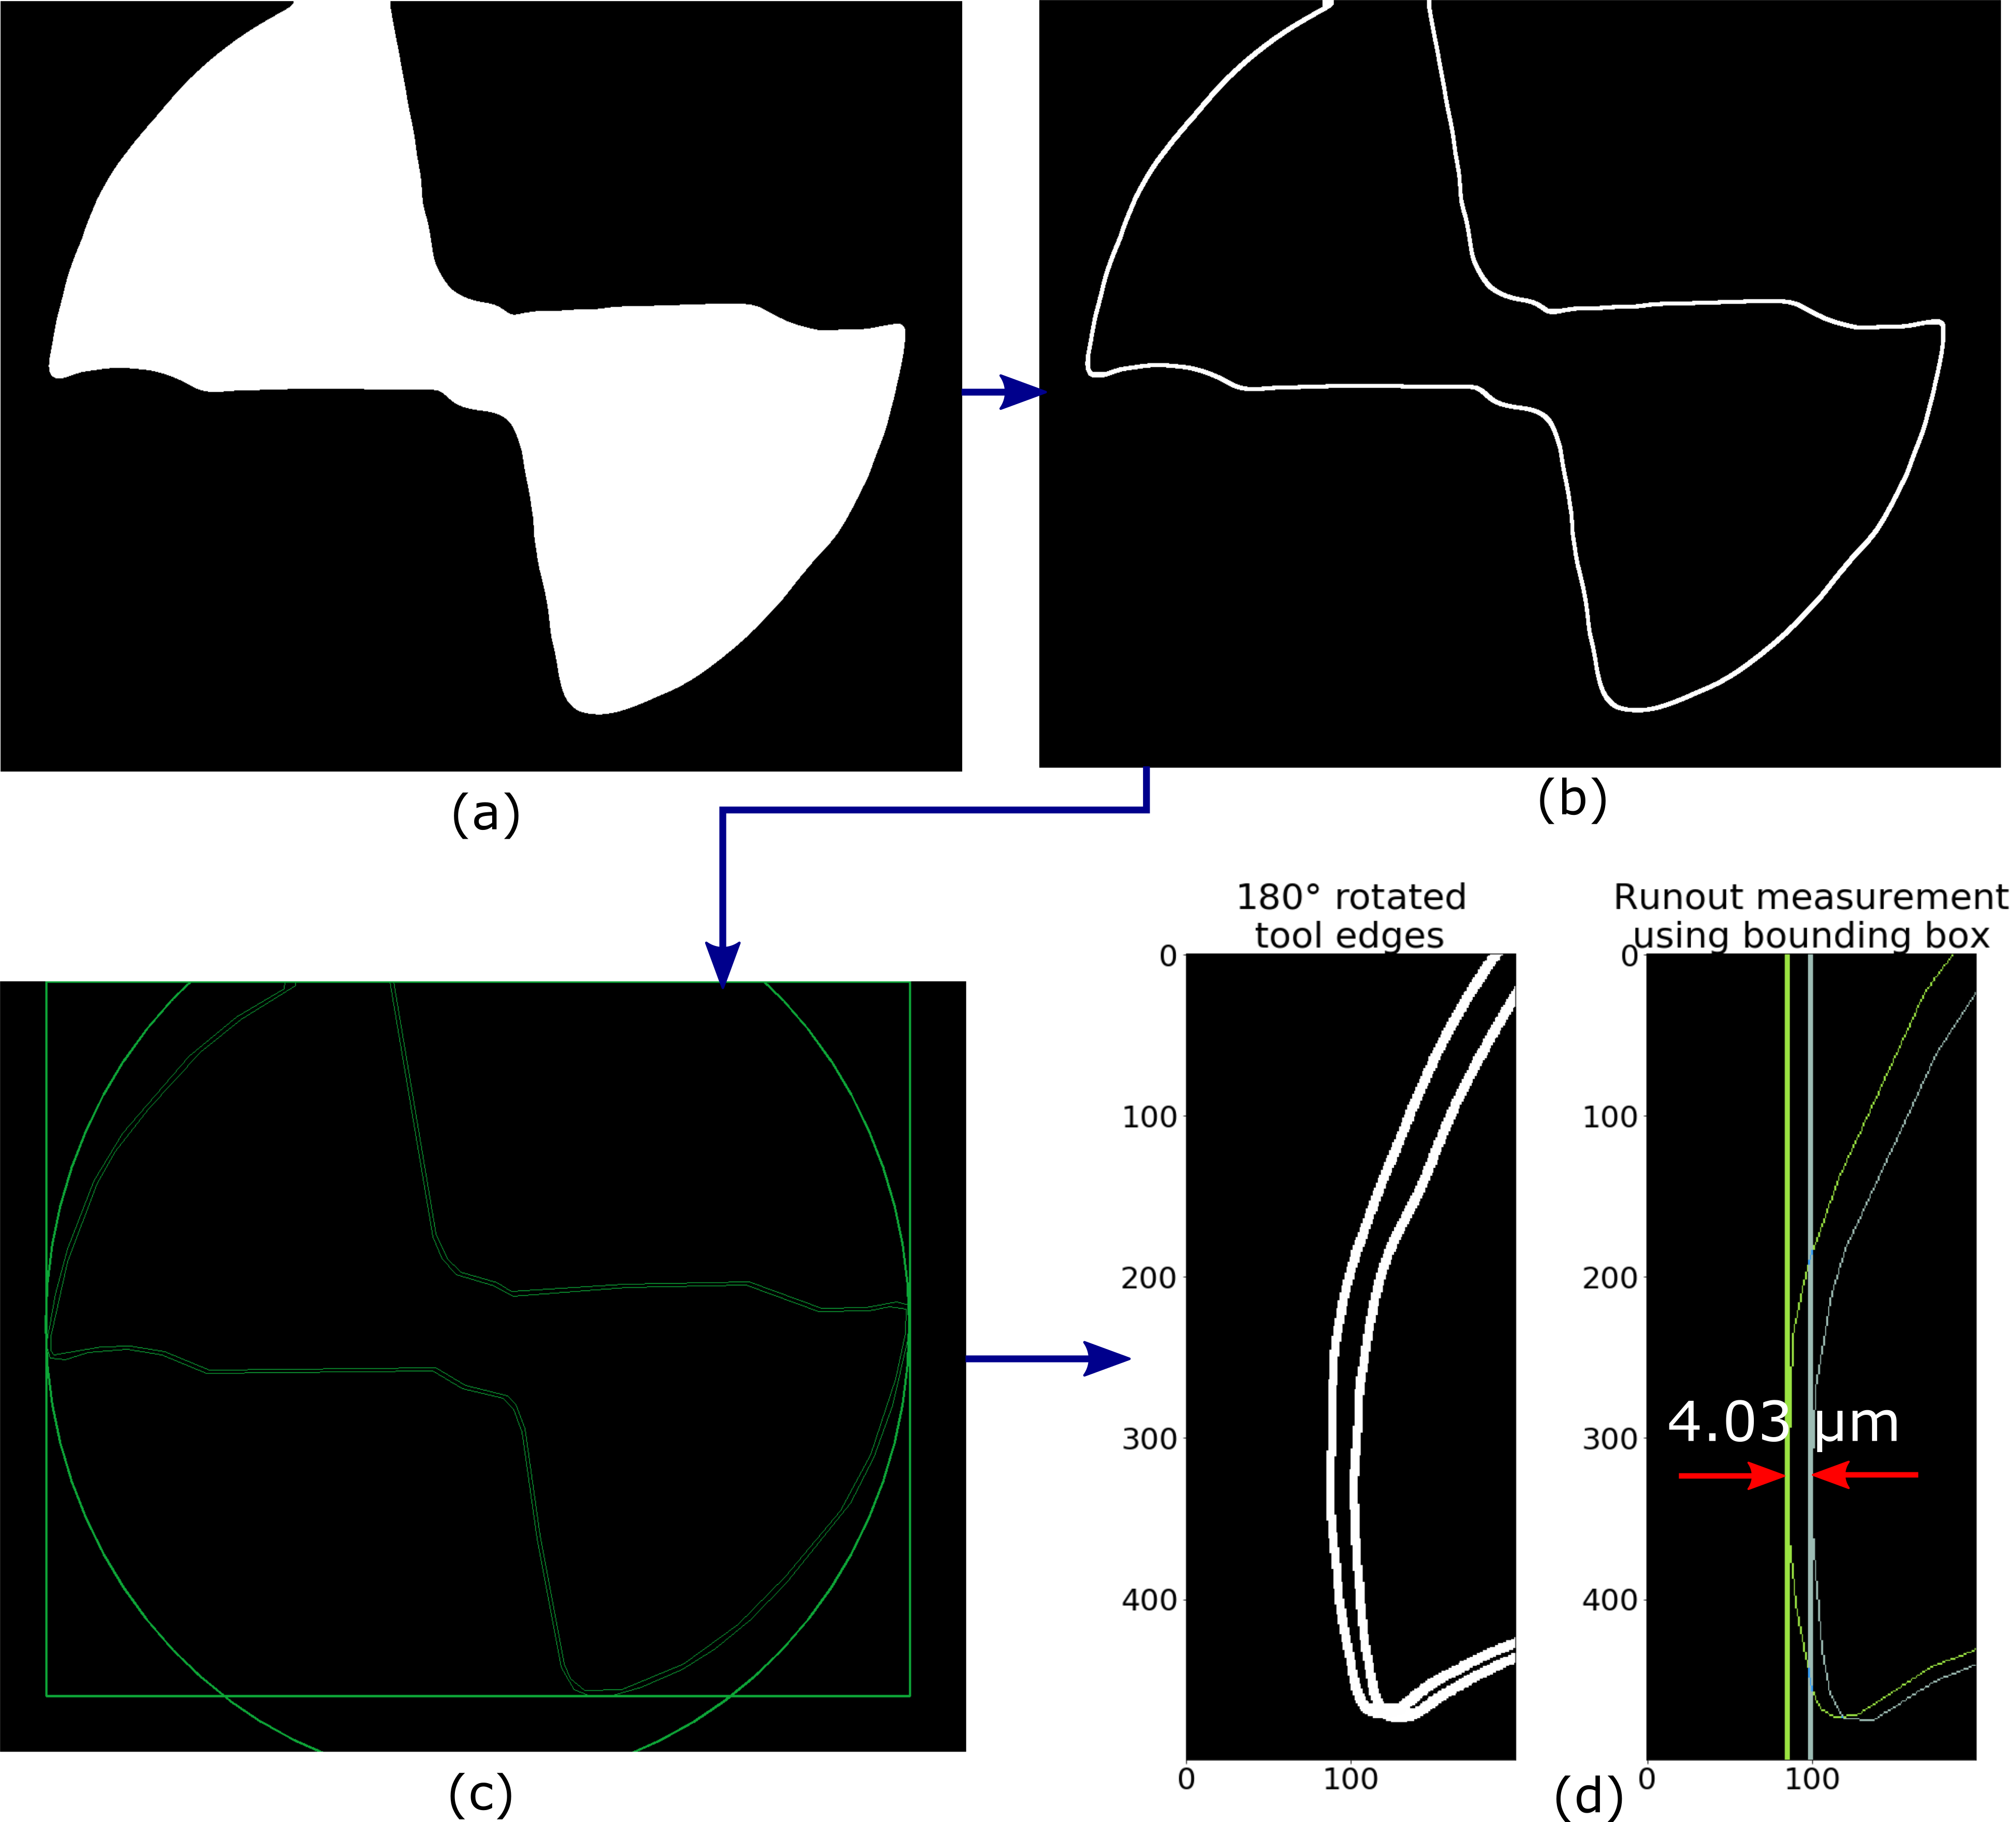
\includegraphics[width=0.7\linewidth]{320.png}
\caption{The process flow to compute static radial tool runout: (a) Binarized tool image (b) Edge detection of the tool (c) Contour and bounding box detection (d) Runout calculation}\label{fig:fig320}
\end{center}
\end{figure}

\subsection{Computing wear classes and remaining-useful-life}\label{sec:sec44}
After obtaining the diameter reduction and area wear values for all the intermediate tool images, the tool state classification was done as described by Eq. \ref{eq:eq32} for diameter reduction and by using Eq. \ref{eq:eq33} for edge area wear. Class 1 defines the rapid initial wear region, Class 2 defines the steady-state wear and Class 3 defines the critical wear to failure region. The remaining-useful-life (RUL) for a particular data-point was computed by identifying the first time instant when the tool in observation reached the end-of-tool-life criteria and then taking a difference with the time instant of that data point. \par

\begin{equation}\label{eq:eq32}
 \makecell{Diameter\,Reduction \\ classification\,criteria} =
 \begin{cases}
   Class\,1 & \text{if diameter reduction $\leq$ $60\mu{m}$} \\
   Class\,2 & \text{if $60\mu{m}$ $<$ diameter reduction $\leq$ $125\mu{m}$} \\
   Class\,3 & \text{if diameter reduction $>$ $125\mu{m}$}
 \end{cases}
\end{equation}

\begin{equation}\label{eq:eq33}
 \makecell{Edge\,Wear\,Area \\ classification\,criteria} =
 \begin{cases}
   Class\,1 & \text{if wear area $\leq$ $5000\mu{m}^2$} \\
   Class\,2 & \text{if $5000\mu{m}^2$ $<$ wear area $\leq$ $15000\mu{m}^2$} \\
   Class\,3 & \text{if wear area $>$ $15000\mu{m}^2$}
 \end{cases}
\end{equation}

The wear state classification and RUL was added to the preprocessed dataset to be used as output labels for model training. At this point, the process parameters pertaining to each data-point in the dataset were also added as input features for the model. \par

%\fi

\section{Model Architectures and Training}\label{chap:model}
The workflow for the model training process is shown in Fig. \ref{fig:fig321}. The two neural-network architectures employed for training are discussed in sec. \ref{sec:sec41} and sec. \ref{sec:sec42}. \par

\begin{figure}[!h]
  \begin{center}
    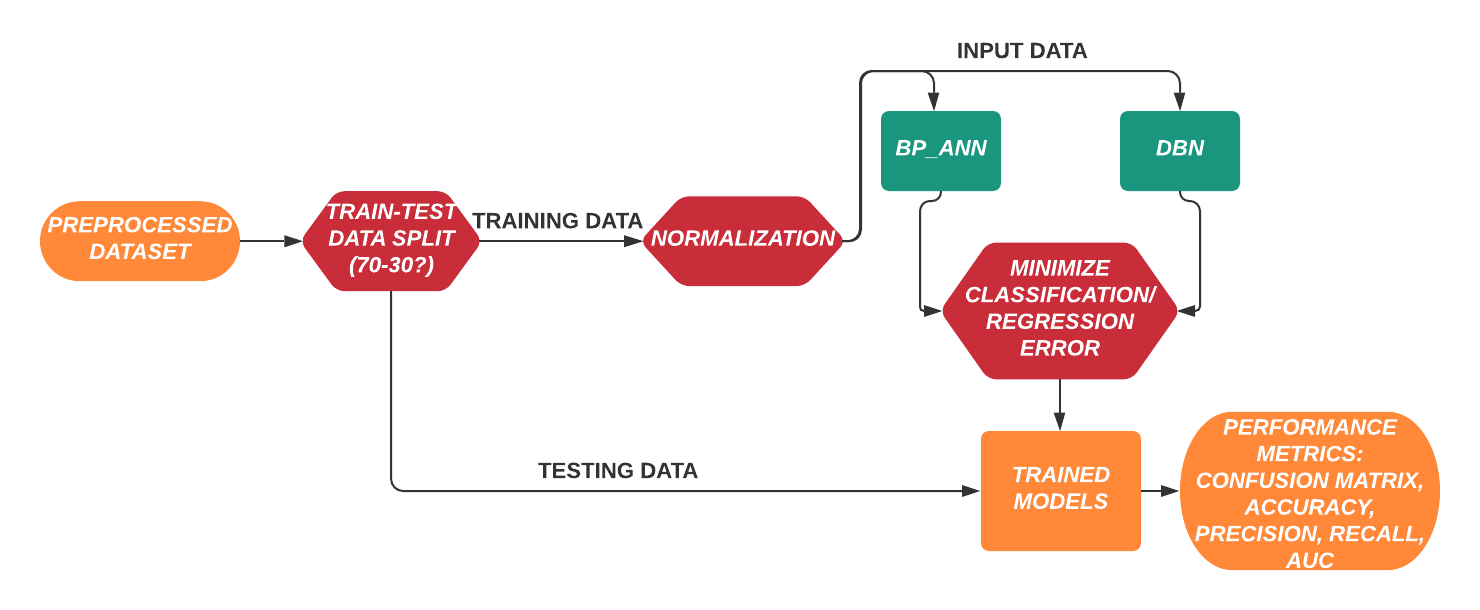
\includegraphics[width=\linewidth]{321.png}
    \caption{The model training process flow}\label{fig:fig321}
  \end{center}
\end{figure}

The dataset obtained after preprocessing was split into train-validation-test sets with the train-test split being 7:3 and train-validation split being 4:1. Separate train-test split was done for each output label: (i) Diameter reduction, (ii) Area wear of edge 1, (iii) Area wear of edge 2 and (iv) Remaining useful life (RUL); and thus four different pairs of training and testing datasets are obtained. The dataset was then normalized to range [0,1] using min-max-scaler. \par

The input data consisted of $63$ features, including the process parameters and the extracted features from the sensor data. The output in each case was dependent on the prediction criteria. For wear state classification based on diameter reduction/area wear of edges, the output labels were one-hot encoded (converted from decimal to binary format) before feeding in for training. For RUL prediction, the output labels were the time to end-of-tool-life (tteotl) value calculated for each datapoint. Subsequently, the artificial neural networks were trained for wear state classification as well as RUL prediction and deep-belief-network was trained for diameter reduction based wear state classification. The architectures implemented for both the models are described below. \par

\subsection{Neural Network}\label{sec:sec41}

The architecture used for training the backpropogated neural-network model is displayed in Fig. \ref{fig:fig322}. \par

\begin{figure}[!h]
  \begin{center}
    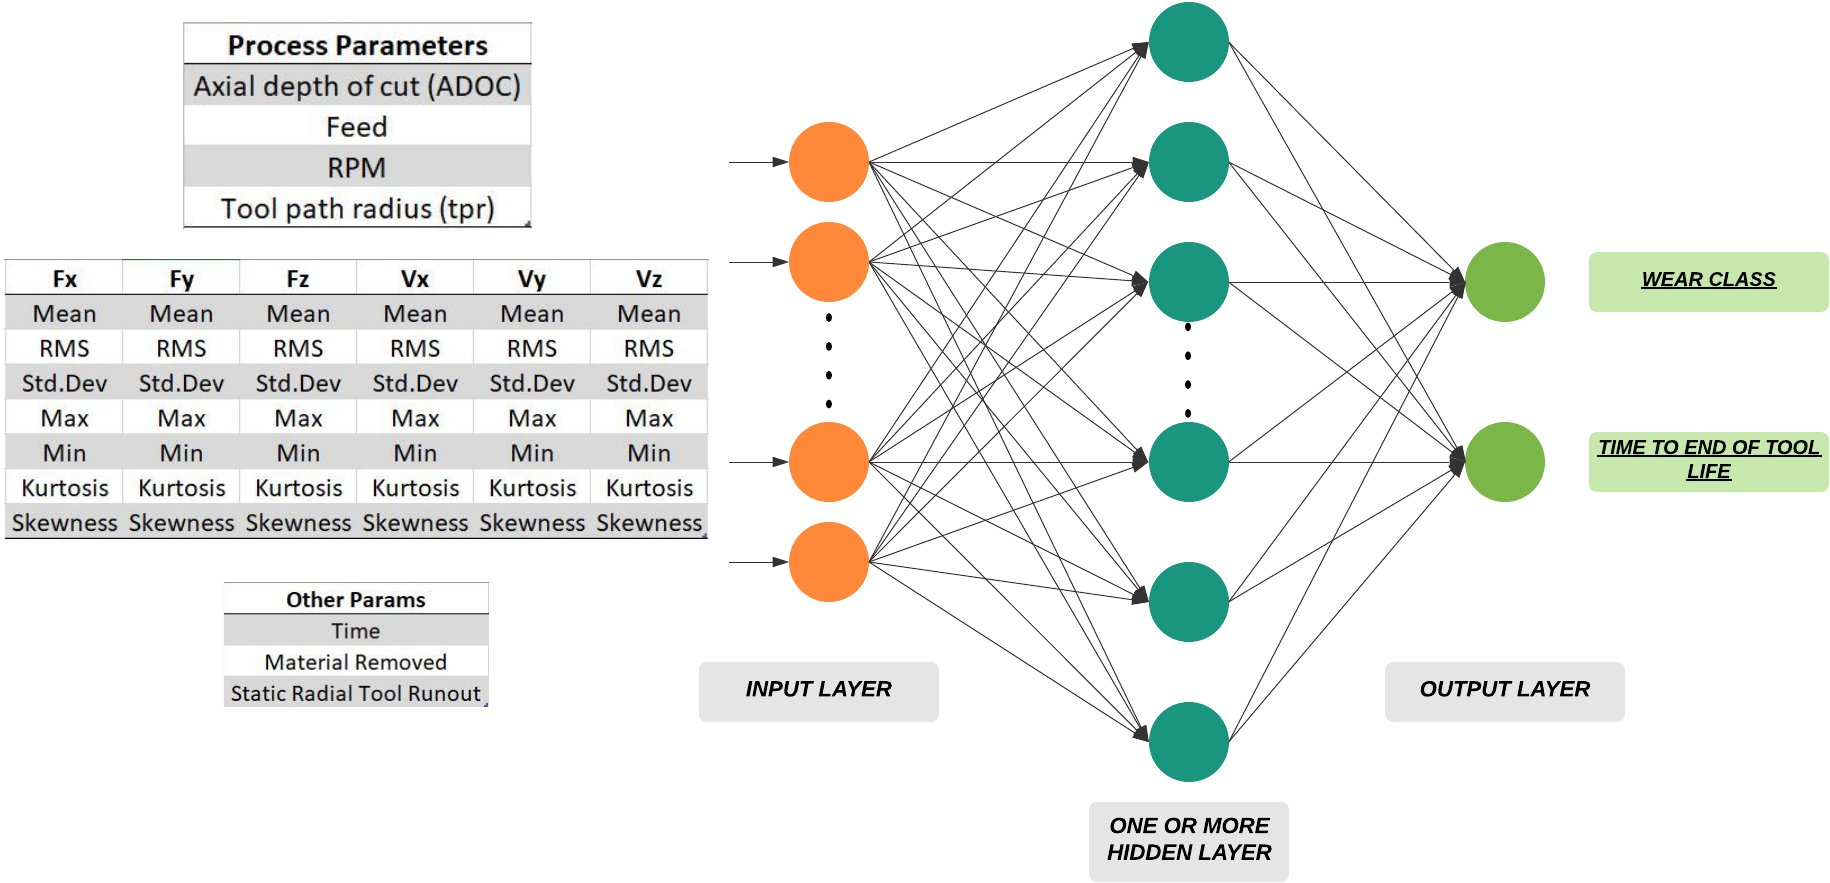
\includegraphics[width=0.9\linewidth]{322.png}
    \caption{Architecture for neural network}\label{fig:fig322}
  \end{center}
\end{figure}

A single dense (fully-connected) hidden layer, with $63$ neurons formed the first layer in the architecture. In the case of regression for RUL prediction, another hidden layer with 200 neurons was added after the first layer. A \emph{relu} activation function was used at the output of the hidden layers. The \emph{relu} function is a piecewise linear function that will output the input directly if is positive and zero otherwise. To prevent overfitting of the training data, a regularization layer with dropout paramter set to 0.2 (20\% of the data would be dropped at random) was added after the hidden layer. Finally, the output layer consisted of 3 neurons, one for each wear state during classification. A softmax activation function was used to convert the logits (a vector of raw, non-normalized predictions that a classification model generates) for each of the wear state into probability values. During regression, the output label was the RUL and was computed directly without the need of any additional activation functions after the output layer. \par

The training was done in mini-batches of size 32 and a total of 100 epochs were used for weight optimization. An epoch is completed when the entire training set passes through the network and contributes to the weight updates. One of the key features of this model training was the usage of Adam optimizer to minimize the classification/regression prediction error. Adam optimization is a stochastic gradient descent (SGD) method that is based on adaptive estimation of first-order and second-order moments. It adapts the learning rate of each weight individually. The moment estimation for the current batch (t) is done as in Eq. \ref{eq:eq34}. Stochastic gradient descent is a technique which randomly picks one data point from the entire dataset to compute the error gradients in each iteration, with the goal of significantly reducing the large computation overhead of the standard gradient descent technique. \par

\begin{subequations}\label{eq:eq34}
  \begin{equation}
    First\,moment:
    \begin{cases}
      Biased & m_t = \beta_1m_{t-1} + (1-\beta_1)g_t \\
      Unbiased & \hat m_t = \frac{m_t}{1-\beta_1^t}
    \end{cases}
  \end{equation}
  \begin{equation}
    Second\,moment:
    \begin{cases}
      Biased & v_t = \beta_2v_{t-1} + (1-\beta_2)g_t^2 \\
      Unbiased & \hat v_t = \frac{v_t}{1-\beta_2^t}
    \end{cases}
  \end{equation}
\end{subequations}

Here, g(t) is the gradient of the current batch and $\beta_1$, $\beta_2$ (and also $\epsilon$) are the control parameters for this optimizer. The values of $\beta_1 = 0.9$ and $\beta_2 = 0.999$ ($\epsilon = 1e-7$) were used. The weight update is then made using the Eq. \ref{eq:eq35} \par

\begin{equation}\label{eq:eq35}
  w_t = w_{t-1} - \eta\frac{\hat m_t}{\sqrt{\hat v_t}+\epsilon}
\end{equation}

Here, $\eta$ is the step size. The trained model is saved alongwith the weights and biases and finally evaluated on the testing set.

\subsection{Deep Belief Network}\label{sec:sec42}
The DBN architecture employed for this study is shown in Fig. \ref{fig:fig324}. The individual components of the architecture and the training process are discussed below.

\begin{figure}[!h]
  \begin{center}
    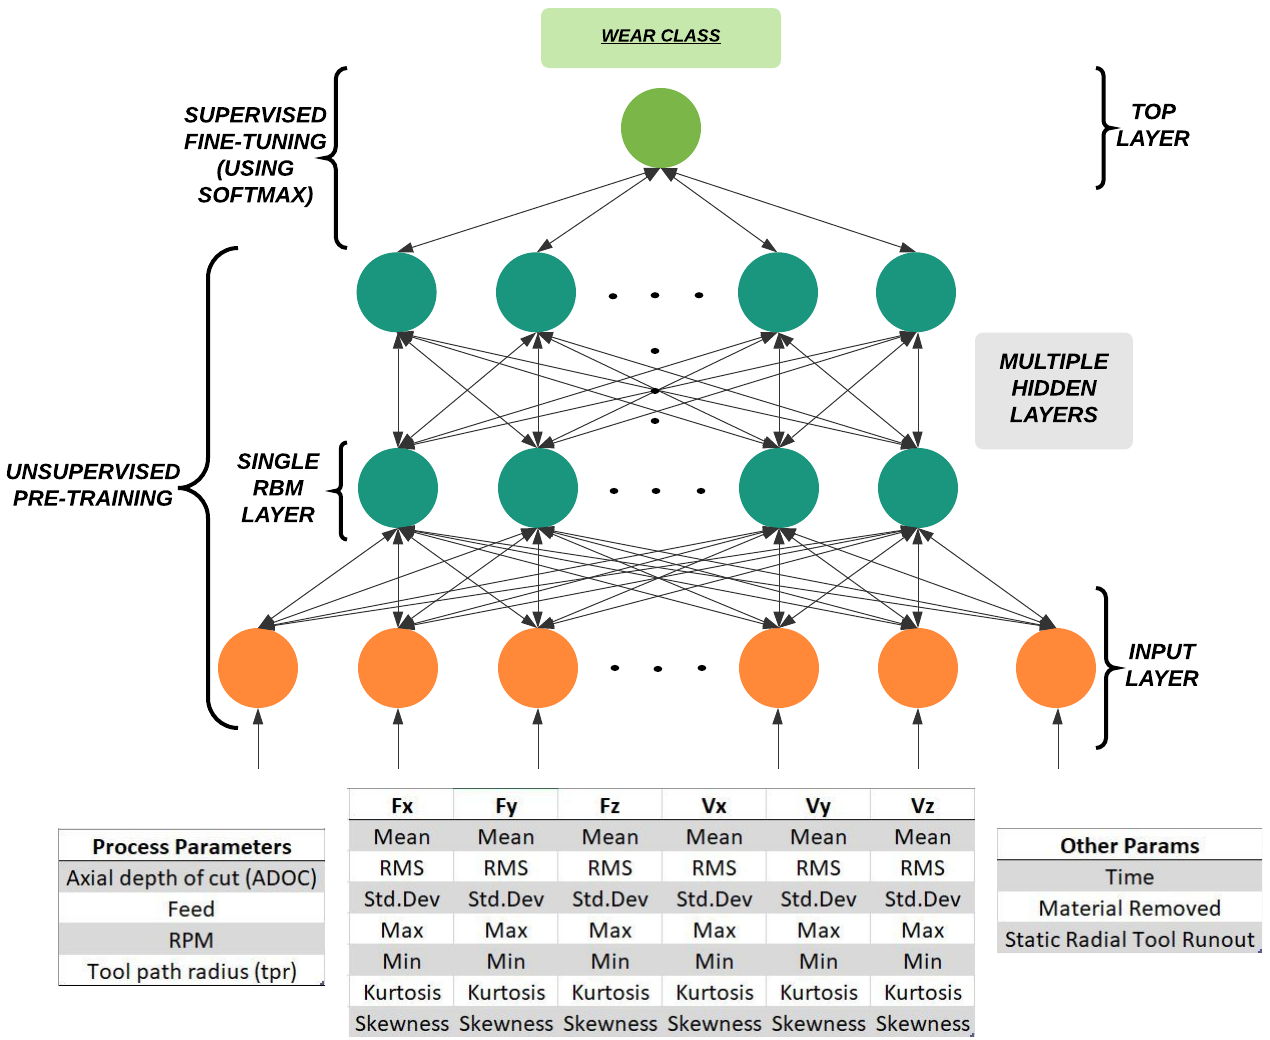
\includegraphics[width=0.75\linewidth]{324.png}
    \caption{Architecture for deep-belief network}\label{fig:fig324}
  \end{center}
\end{figure}

Deep Belief Networks employ a hierarchial structure with multiple stacked restricted boltzmann machines (RBMs) (Fig. \ref{fig:fig323}(a)) and use a layer-by-layer learning technique followed by a fine-tuning procedure. Every layer in a deep belief network (Fig. \ref{fig:fig323}(b)), except the input and output, has a double function. It serves as a hidden layer to the previous layer and as a visible layer to the next layer. The training process consists of a pre-training, fine-tuning and prediction. \par

\begin{figure}[!h]
  \begin{center}
    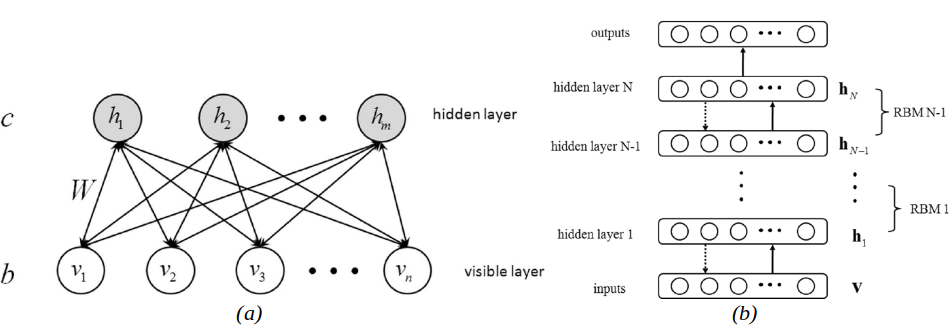
\includegraphics[width=\linewidth]{323.png}
    \caption{The structure of deep belief networks (a) restriced boltzmann machine (RBM) (b) stack of multiple RBMs to form a DBN \cite{CITE9}}\label{fig:fig323}
  \end{center}
\end{figure}

RBMs (Fig. \ref{fig:fig323}(a)) are a type of generative stochastic artificial neural network and are effective in feature extraction for initializing the feed-forward neural network. There are two layers in an RBM namely the visible and the hidden layers and each neuron in these layers has a binary value (0 or 1). Each neuron in the visible layer is connected to the neurons in the hidden layer in an undirected way with no connections within a layer. Each connection has a weight associated with it and is denoted by \textbf{w} = ${w\textsubscript{ij}}$ such that it is the undirected weight associated with hidden neuron {$h\textsubscript{j}$} and visible neuron $v\textsubscript{i}$. The biases associated with the visible and hidden neurons are denoted by vectors \textbf{b} and \textbf{c}, respectively. The set of parameters including the weights and biases is denoted by $\theta$ \cite{CITE9}. The probability of neuron having value 0 or 1 is calculated based on the energy Eq. \ref{eq:eq36}. The energy of the joint configuration is given by Eq. \ref{eq:eq37}, where $I$ and $J$ are the number of visible and hidden units. \par

\begin{subequations}\label{eq:eq36}
  \begin{equation}
    For\: hidden\: neuron\: h_j: E_j = \sum_{i=1}^{n} w_{ij}v_i + c_j\label{eq:eq4}
  \end{equation}
  \begin{equation}
    For\: visible\: neuron\: v_i: E_i = \sum_{j=1}^{m} w_{ij}h_j + b_i\label{eq:eq5}
  \end{equation}
\end{subequations}

\begin{equation}\label{eq:eq37}
  E(\mathbf{v},\mathbf{h},\theta) = -\sum_{i=1}^{I}\sum_{j=1}^{J}w_{ij}v_ih_j-\sum_{i=1}^{I}b_iv_i-\sum_{j=1}^{J}c_ih_j
\end{equation}

The model assigns a probability value to a visible vector (\textbf{v}) as given by Eq. \ref{eq:eq38}. The final values of the neurons in the visible vector are determined by choosing a random number (u) to define a step function for h\textsubscript{j}, where it is equal to 1 if P(h\textsubscript{j} = 1) $\geq$ u, and 0 otherwise.

\begin{equation}\label{eq:eq38}
P(\mathbf{v}; \theta) = \sum_{\mathbf{h}}P(\mathbf{v},\mathbf{h};\theta)  = \frac{1}{\sum_{\mathbf{h}} \sum_{\mathbf{v}} e^{-E(\mathbf{v},\mathbf{h};\theta)}} \sum_{\mathbf{h}} (e^{\mathbf{v^Twh}+\mathbf{b^Tv}+\mathbf{c^Th}})
\end{equation}

The pre-training involves using the stochastic gradient descent (SGD) technique to optimize the weights and the biases by calculating the negative log probability (Eq. \ref{eq:eq39} \cite{CITE9}). Each hidden layer is trained using the activation probabilities of the hidden layer of the lower RBM as input data, and its own output serves as the input for the upper RBM. For this unsupervised, layer-by-layer training, a total of 10 epochs demonstrated optimal performance. \par

\begin{equation}\label{eq:eq39}
  \resizebox{0.5\textwidth}{!}
  {$
  \begin{cases}
    \frac{\partial{lnP(\mathbf{v};\theta)}}{\partial{w_{ij}}} = \langle{v_ih_j}\rangle_{data} - \langle{v_ih_j}\rangle_{model} \\\\
    \frac{\partial{lnP(\mathbf{v};\theta)}}{\partial{\mathbf{c}}} = \langle{h_j}\rangle_{data} - \langle{h_j}\rangle_{model} \\\\
    \frac{\partial{lnP(\mathbf{v};\theta)}}{\partial{\mathbf{b}}} = \langle{v_i}\rangle_{data} - \langle{h_i}\rangle_{model} \\
  \end{cases}
  $}
\end{equation}

A softmax layer was added after the final hidden layer to convert the raw output values to probabilities of wear classes. The fine-tuning of model weights and biases involves using backpropogation which forms the supervised learning step to minimize the classification error.

%==========================================================================================================%
%\iffalse
\section{Results and Discussions}\label{chap:results}

This section is divided into two parts: Section \ref{sec:sec51} discusses the results from the analysis done based on the experimental procedure. Section \ref{sec:sec52} details the model performances and the characteristics of the prediction results. \par

\subsection{Experimental results}\label{sec:sec51}
The tool wear progression and force analysis is discussed from an overall point of view as well as in terms of variation with tool path radius. The tool ids (Table \ref{tab:T35}): T80, T82, T83, T85 and T86 broke prematurely while T79, T81 and T84 reached the end-of-life criteria. Tool ids T82, T85 and T86 suffered catastrophic failure after only a few seconds of machining. \par

\subsubsection{Variation of static runout and peak-to-peak forces}
The analysis of the pre-machining tool images, after installing in the machining center, yielded the static radial tool runout. The runout values measured at different angles and the mean runout value for each experiment are described in Table \ref{tab:T51}. The calculated values of static radial tool runout for $T83$ (7.03 $\mu{m}$) and $T86$ (5.57 $\mu{m}$) were considerably large. This could be a potential reason for their catastrophic failure. \par


\begin{minipage}{\linewidth}
  \captionof{table}{Static radial tool runout} \label{tab:T51}
  \centering
  \resizebox{0.6\textwidth}{!}{
    \begin{tabular}{ c | c c c c c c c }
    	\hline
      \makecell{Tool \\ No} & \makecell{$val_1$ \\ $(\mu{m})$}	& \makecell{$val_2$ \\ $(\mu{m})$} & \makecell{$val_3$ \\ $(\mu{m})$} & \makecell{$val_4$ \\ $(\mu{m})$} & \makecell{$val_5$ \\ $(\mu{m})$} & \makecell{$val_6$ \\ $(\mu{m})$} &	\makecell{Average \\ $(\mu{m})$} \\
    	\hline\hline
     	$T79$ & $1.95$ & $4.03$ & $2.21$ & $-$ & $-$ & $-$ & $2.73$ \\
     	\hline
     	$T80$ & $6.29$ & $6.82$ & $6.27$ & $8.39$ & $8.24$ & $8.67$ & $7.45$ \\
     	\hline
      $T81$ & $2.13$ & $2.41$ & $2.5$ & $2.17$ & $2.77$ & $-$ & $2.39$ \\
      \hline
      $T82$ & $5.2$ & $5.12$ & $5.3$ & $5.43$ & $5.79$ & $-$ & $5.37$ \\
      \hline
      $T83$ & $7.81$ & $7.2$ & $7.52$ & $4.81$ & $7.09$ & $7.78$ & $7.03$ \\
      \hline
      $T84$ & $3.38$ & $3.28$ & $4.88$ & $4.36$ & $4.31$ & $4.67$ & $4.15$ \\
      \hline
      $T85$ & $6.3$ & $5.58$ & $5.5$ & $6.07$ & $5.44$ & $6.01$ & $5.82$ \\
      \hline
      $T86$ & $5.39$ & $5.75$ & $5.24$ & $5.44$ & $5.77$ & $5.87$ & $5.57$ \\
      \hline
    \end{tabular}}
\end{minipage} \\\\

The peak-to-peak force was analyzed for the entire duration of machining for all the experiments as shown in Fig. \ref{fig:fig51}. A sudden drop in force values was observed around 700 seconds of machining for T79 (Fig. \ref{fig:fig51}(a)) indicating that the tool entered a secondary steady state region before reaching end-of-life. Forces for T81 (Fig. \ref{fig:fig51}(c)) showed a higher magnitude in the x-direction whereas for T80, T83 and T84 (Fig. \ref{fig:fig51}(b,e,f)) the magnitude in the y-direction was higher than the other directions. Fig. \ref{fig:fig51}(d,g,h) shows a similar rate of increase in force magnitude in all the three directions before the catastrophic failure of the tools. \par

\begin{figure}[!h]
  \begin{center}
    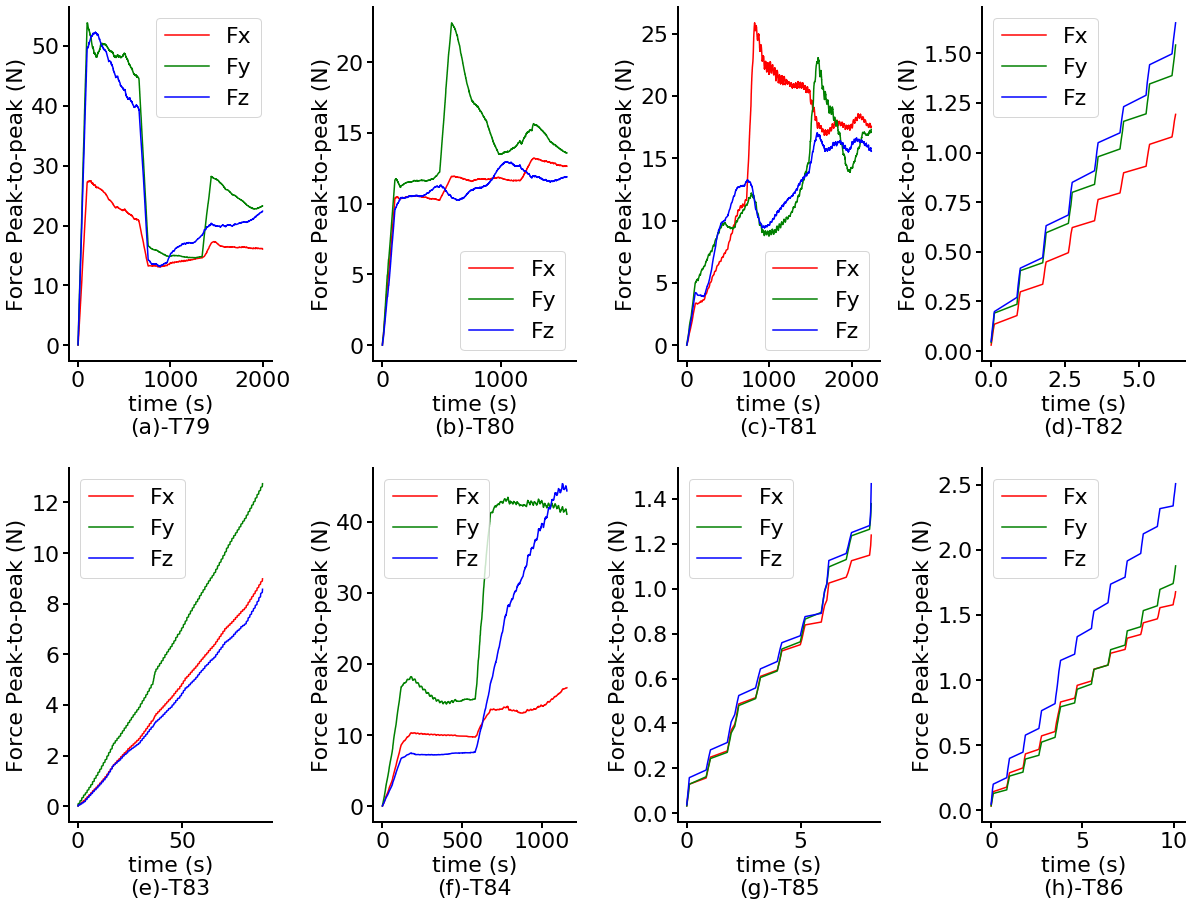
\includegraphics[width=\linewidth]{51.png}
    \caption{Peak-to-peak force variations: ([a-h] for individual experiments)}\label{fig:fig51}
  \end{center}
\end{figure}

\subsubsection{Variation of tool wear with tool path radius}
Three different metrics were used to quantify tool state: (i) Diameter reduction; (ii) Chipped area of edge 1; (iii) Chipped area of edge 2. The individual edge-wear quantification helps in better understanding the tool state. The wear progression curves, in terms of diameter reduction with distance for different tpr is shown in Fig. \ref{fig:fig52}. For tpr of 250 $\mu{m}$ (Fig. \ref{fig:fig52}(a)), the tools entered the steady state region after machining a distance of 100-150 mm. However for tpr of 500 $\mu{m}$ (Fig. \ref{fig:fig52}(b)) the tools (T83 and T84) were able machine a distance of 60-100 mm before entering steady state region (T84) or breaking (T83). On the other hand, T82 entered the critical wear region after machining only 10-15 mm and then broke. The diameter reduction (Fig. \ref{fig:fig52}(c)), after having machined only 5-10 mm, was even more severe for tpr of 750 $\mu{m}$. This indicates that the rate of tool wear progressively increases with increas in tool path radius. \par

\begin{figure}[!h]
  \begin{center}
    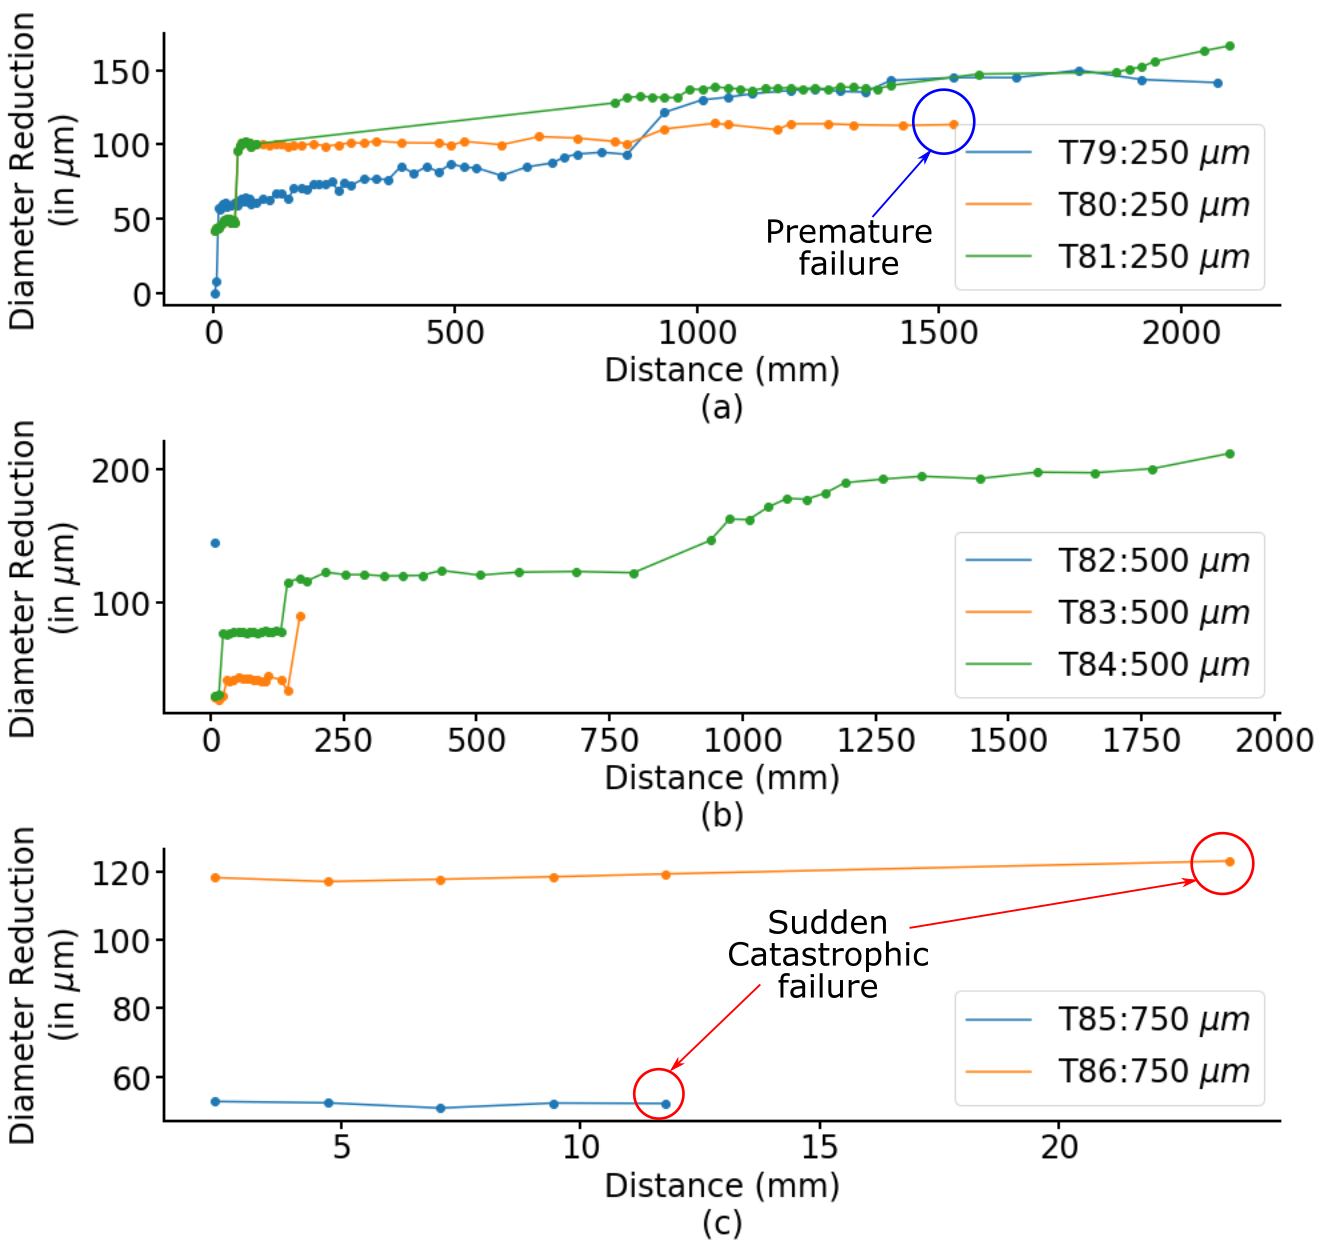
\includegraphics[width=\linewidth]{52.png}
    \caption{Variation in diameter reduction with distance: (a) 250 $\mu{m}$ tpr (b) 500 $\mu{m}$ tpr (c) 750 $\mu{m}$ tpr}\label{fig:fig52}
  \end{center}
\end{figure}

The tool condition for each of the three tool path radii at different wear stages (\RomanNumeralCaps{1} - Fresh tool, \RomanNumeralCaps{2} - Rapid initial wear, \RomanNumeralCaps{3} - Steady state wear and \RomanNumeralCaps{4} - Before breakage) is shown in Fig. \ref{fig:fig53}. The variation in tool condition with 250 $\mu{m}$ tpr  showed rounding of cutting edges followed by severe flank wear (Fig. \ref{fig:fig53}(a-\RomanNumeralCaps{2},\RomanNumeralCaps{3})) before breakage. Significant adhesive wear (Fig. \ref{fig:fig53}(b-\RomanNumeralCaps{2},\RomanNumeralCaps{4})) was observed for 500 $\mu{m}$ tpr before breakage. For 750 $\mu{m}$ tpr, excessive chipping of edges (Fig. \ref{fig:fig53}(c-\RomanNumeralCaps{2})) along with some adhesion was observed.

\begin{figure}[!h]
  \begin{center}
    \includegraphics[width=\linewidth]{53.png}
    \caption{Tool images at different stages for different tpr: (a) 250 $\mu{m}$ tpr (b) 500 $\mu{m}$ tpr (c) 750 $\mu{m}$ tpr}\label{fig:fig53}
  \end{center}
\end{figure}

The analysis of individual edge wear for different tpr (Fig. \ref{fig:fig54}) shows that, at any given instant, there is only one cutting edge in contact with the workpiece. For both 250 $\mu{m}$ tpr (Fig. \ref{fig:fig54}(a)) and 500 $\mu{m}$ tpr (Fig. \ref{fig:fig54}(b)), the first shift of contact from edge 1 to edge 2 was observed within 70-100 seconds of machining. The subsequent shifts varied from experiment to experiment. For 750 $\mu{m}$ tpr (Fig. \ref{fig:fig54}(c)) no switch was detected as the tools suffered a catastrophic failure after machining for only 10-15 seconds.

\begin{figure}[!h]
  \begin{center}
    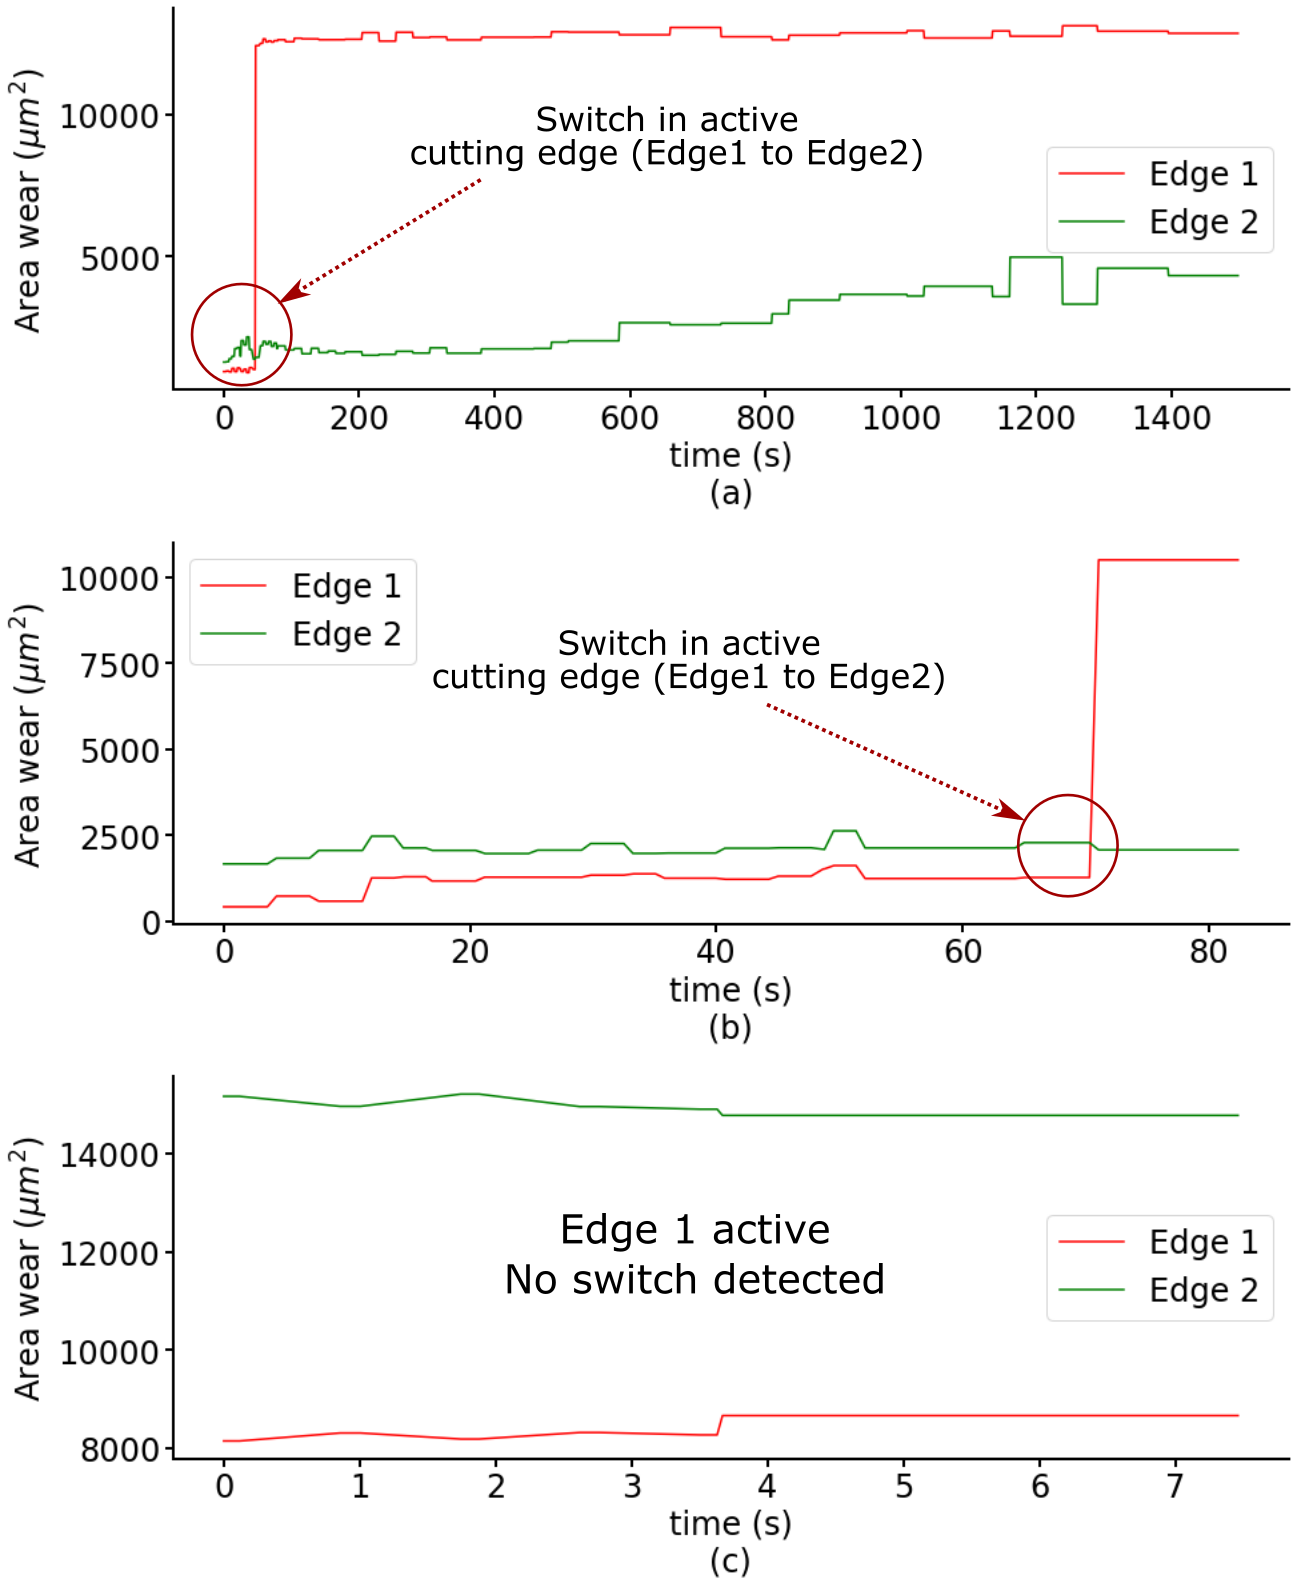
\includegraphics[width=0.7\linewidth]{54.png}
    \caption{Variation of area wear of individual cutting edges with time for different tpr: (a) 250 $\mu{m}$ tpr (b) 500 $\mu{m}$ tpr (c) 750 $\mu{m}$ tpr}\label{fig:fig54}
  \end{center}
\end{figure}


\subsection{Model performances and predictions}\label{sec:sec52}
Two predictive models were used for training including the ANN and DBN. The training set consisted of 18737 data points while the testing set consisted of 10038 data points for both the models. The performances of both ANN and DBN are evaluated and discussed in the following sections. \par

\subsubsection{ANN performance}
The ANN architecture involved 4 different output parameters. The diameter reduction and chipping area of each cutting edge were used for wear state classification. Fig. \ref{fig:fig55}(a) shows the evolution of various performance metrics as the model is trained. Fig. \ref{fig:fig55}(a-\RomanNumeralCaps{1}) shows the variation of the categorical cross-entropy loss with training epochs. Categorical cross-entropy loss function is a measure of how distinguishable two discrete probability distributions are from each other. Higher value of loss indicates that the classification model is not able to accurately distinguish between different classes. The AUC curve (Fig. \ref{fig:fig55}(a-\RomanNumeralCaps{2})) is another measure of separability where a higher value indicates that the model is able to accurately distinguish between classes. Precision (Fig. \ref{fig:fig55}(a-\RomanNumeralCaps{3})) is defined as the fraction of predictions for a particular class that were actually correct. Finally, recall (Fig. \ref{fig:fig55}(a-\RomanNumeralCaps{4})) is defined as the fraction of the total number of data points belonging to a particular class that were accurately predicted. The remaining-useful-life (RUL) was predicted using a regression model and the statistics used include mean squared error (b-\RomanNumeralCaps{1},\RomanNumeralCaps{2}), mean absolute error (b-\RomanNumeralCaps{3}) and the cosine-value (b-\RomanNumeralCaps{4}) (Fig. \ref{fig:fig55}(b)). A larger cosine-value indicates a higher correlation between predicted and actual values.

\begin{figure}[!h]
  \begin{center}
    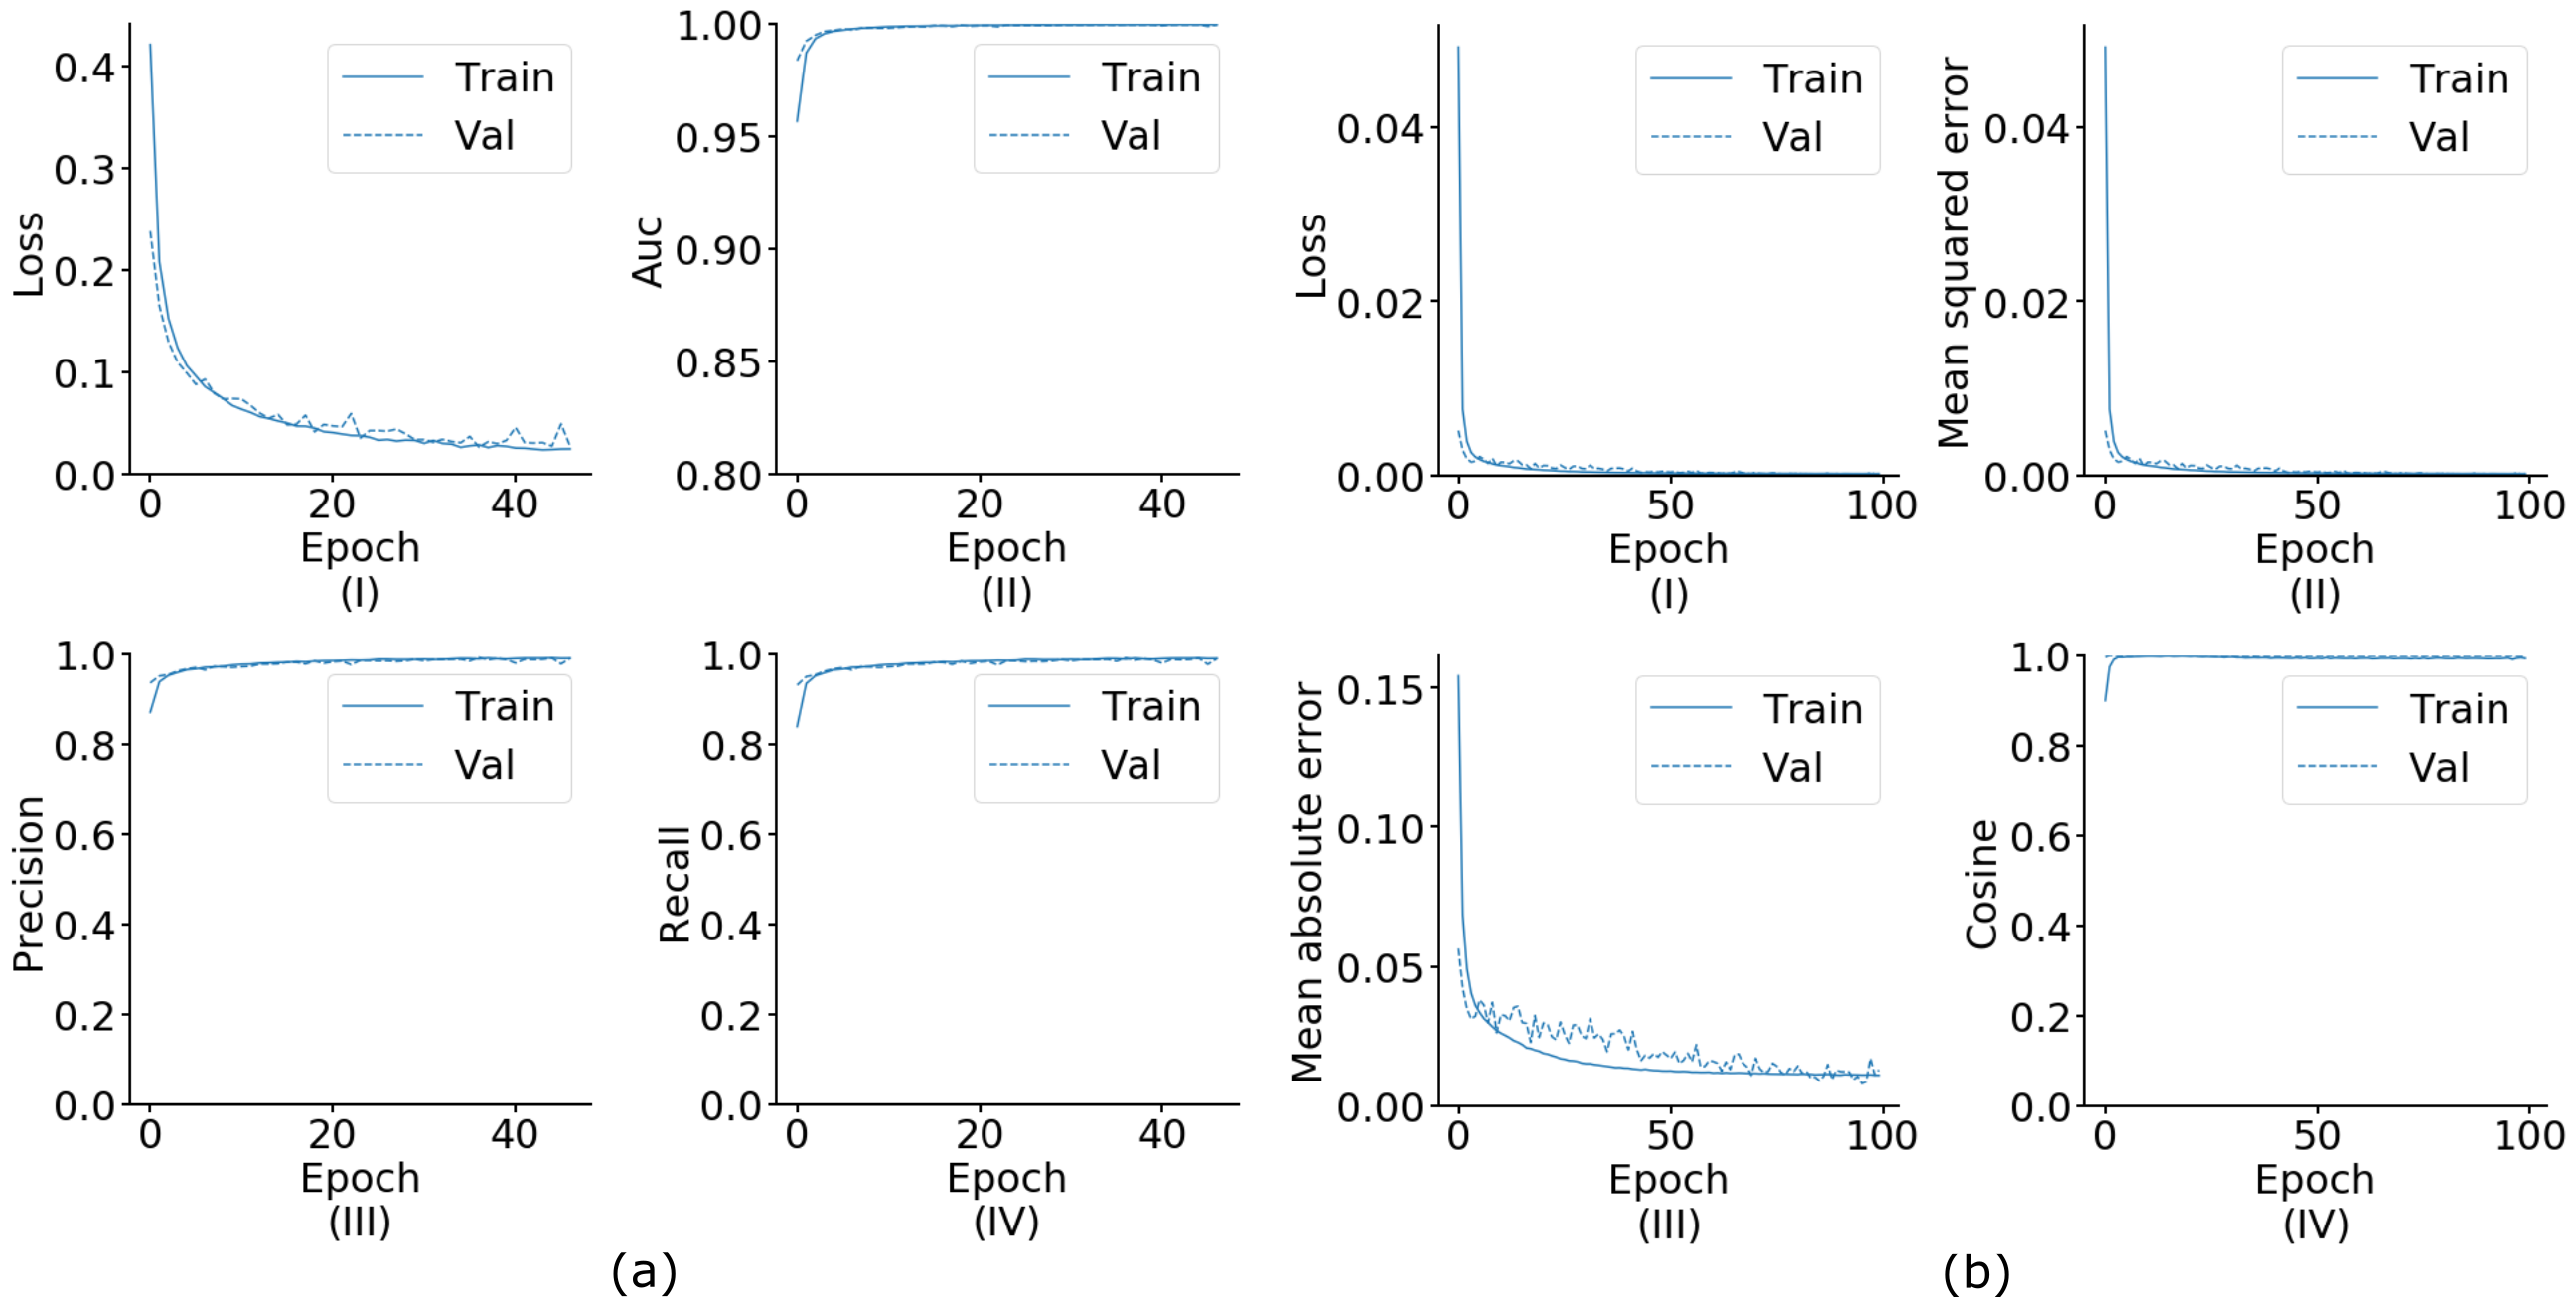
\includegraphics[width=\linewidth]{55.png}
    \caption{Training statistics for ANN  (a) Diameter reduction (b) RUL}\label{fig:fig55}
  \end{center}
\end{figure}

The model was then evaluated on unseen testing data and the results obtained are detailed in Table. \ref{tab:T52}. It is observed that the ANN is able to predict wear state related to each cutting edge with a slightly better accuracy than the state related to diameter reduction. This can be expected as the diameter reduction metric is a function of both the cutting edge wear values and therefore would have a compounded error in prediction than the individual edge wear. \par

\begin{minipage}{\linewidth}
  \captionof{table}{ANN Model performance metric on testing dataset} \label{tab:T52}
  \centering
  \resizebox{0.7\textwidth}{!}{
    \begin{tabular}{ c | c c c c c c }
    	\hline
      \makecell{Output \\ Label} & Accuracy	& Precision & Recall & MSE & MAE & Cosine \\
    	\hline\hline
     	Diameter Reduction & $0.9873$ & $0.9812$ & $0.9808$ & $-$ & $-$ & $-$ \\
     	\hline
     	Area Wear E1 & $0.9945$ & $0.9918$ & $0.9917$ & $-$ & $-$ & $-$ \\
     	\hline
      Area Wear E2 & $0.9923$ & $0.9885$ & $0.9884$ & $-$ & $-$ & $-$ \\
      \hline
      RUL & $-$ & $-$ & $-$ & $11.38$ & $0.6451$ & $0.9634$ \\
      \hline
    \end{tabular}}
\end{minipage} \\\\

The confusion matrices (displaying variation of true label with predicted label) pertaining to the three output labels are shown in Fig. \ref{fig:fig56}. For the diameter reduction output label (Fig. \ref{fig:fig56}(a)), 263 out of 304 labels in the initial wear region, 5392 out of 5426 labels in the steady state region and 4302 out of 4308 labels in the critical wear region were accurately classified. For the edge 1 area wear output label (Fig. \ref{fig:fig56}(a)), 1648 out of 1667 labels in the initial wear region, 6949 out of 6973 labels in the steady state region and 1292 out of 1398 labels in the critical wear region were accurately classified. For the edge 2 area wear output label (Fig. \ref{fig:fig56}(a)), 3797 out of 3813 labels in the initial wear region, all the labels in the steady state region and 1482 out of 1487 labels in the critical wear region were accurately classified. \par


\begin{figure}[!h]
  \begin{center}
    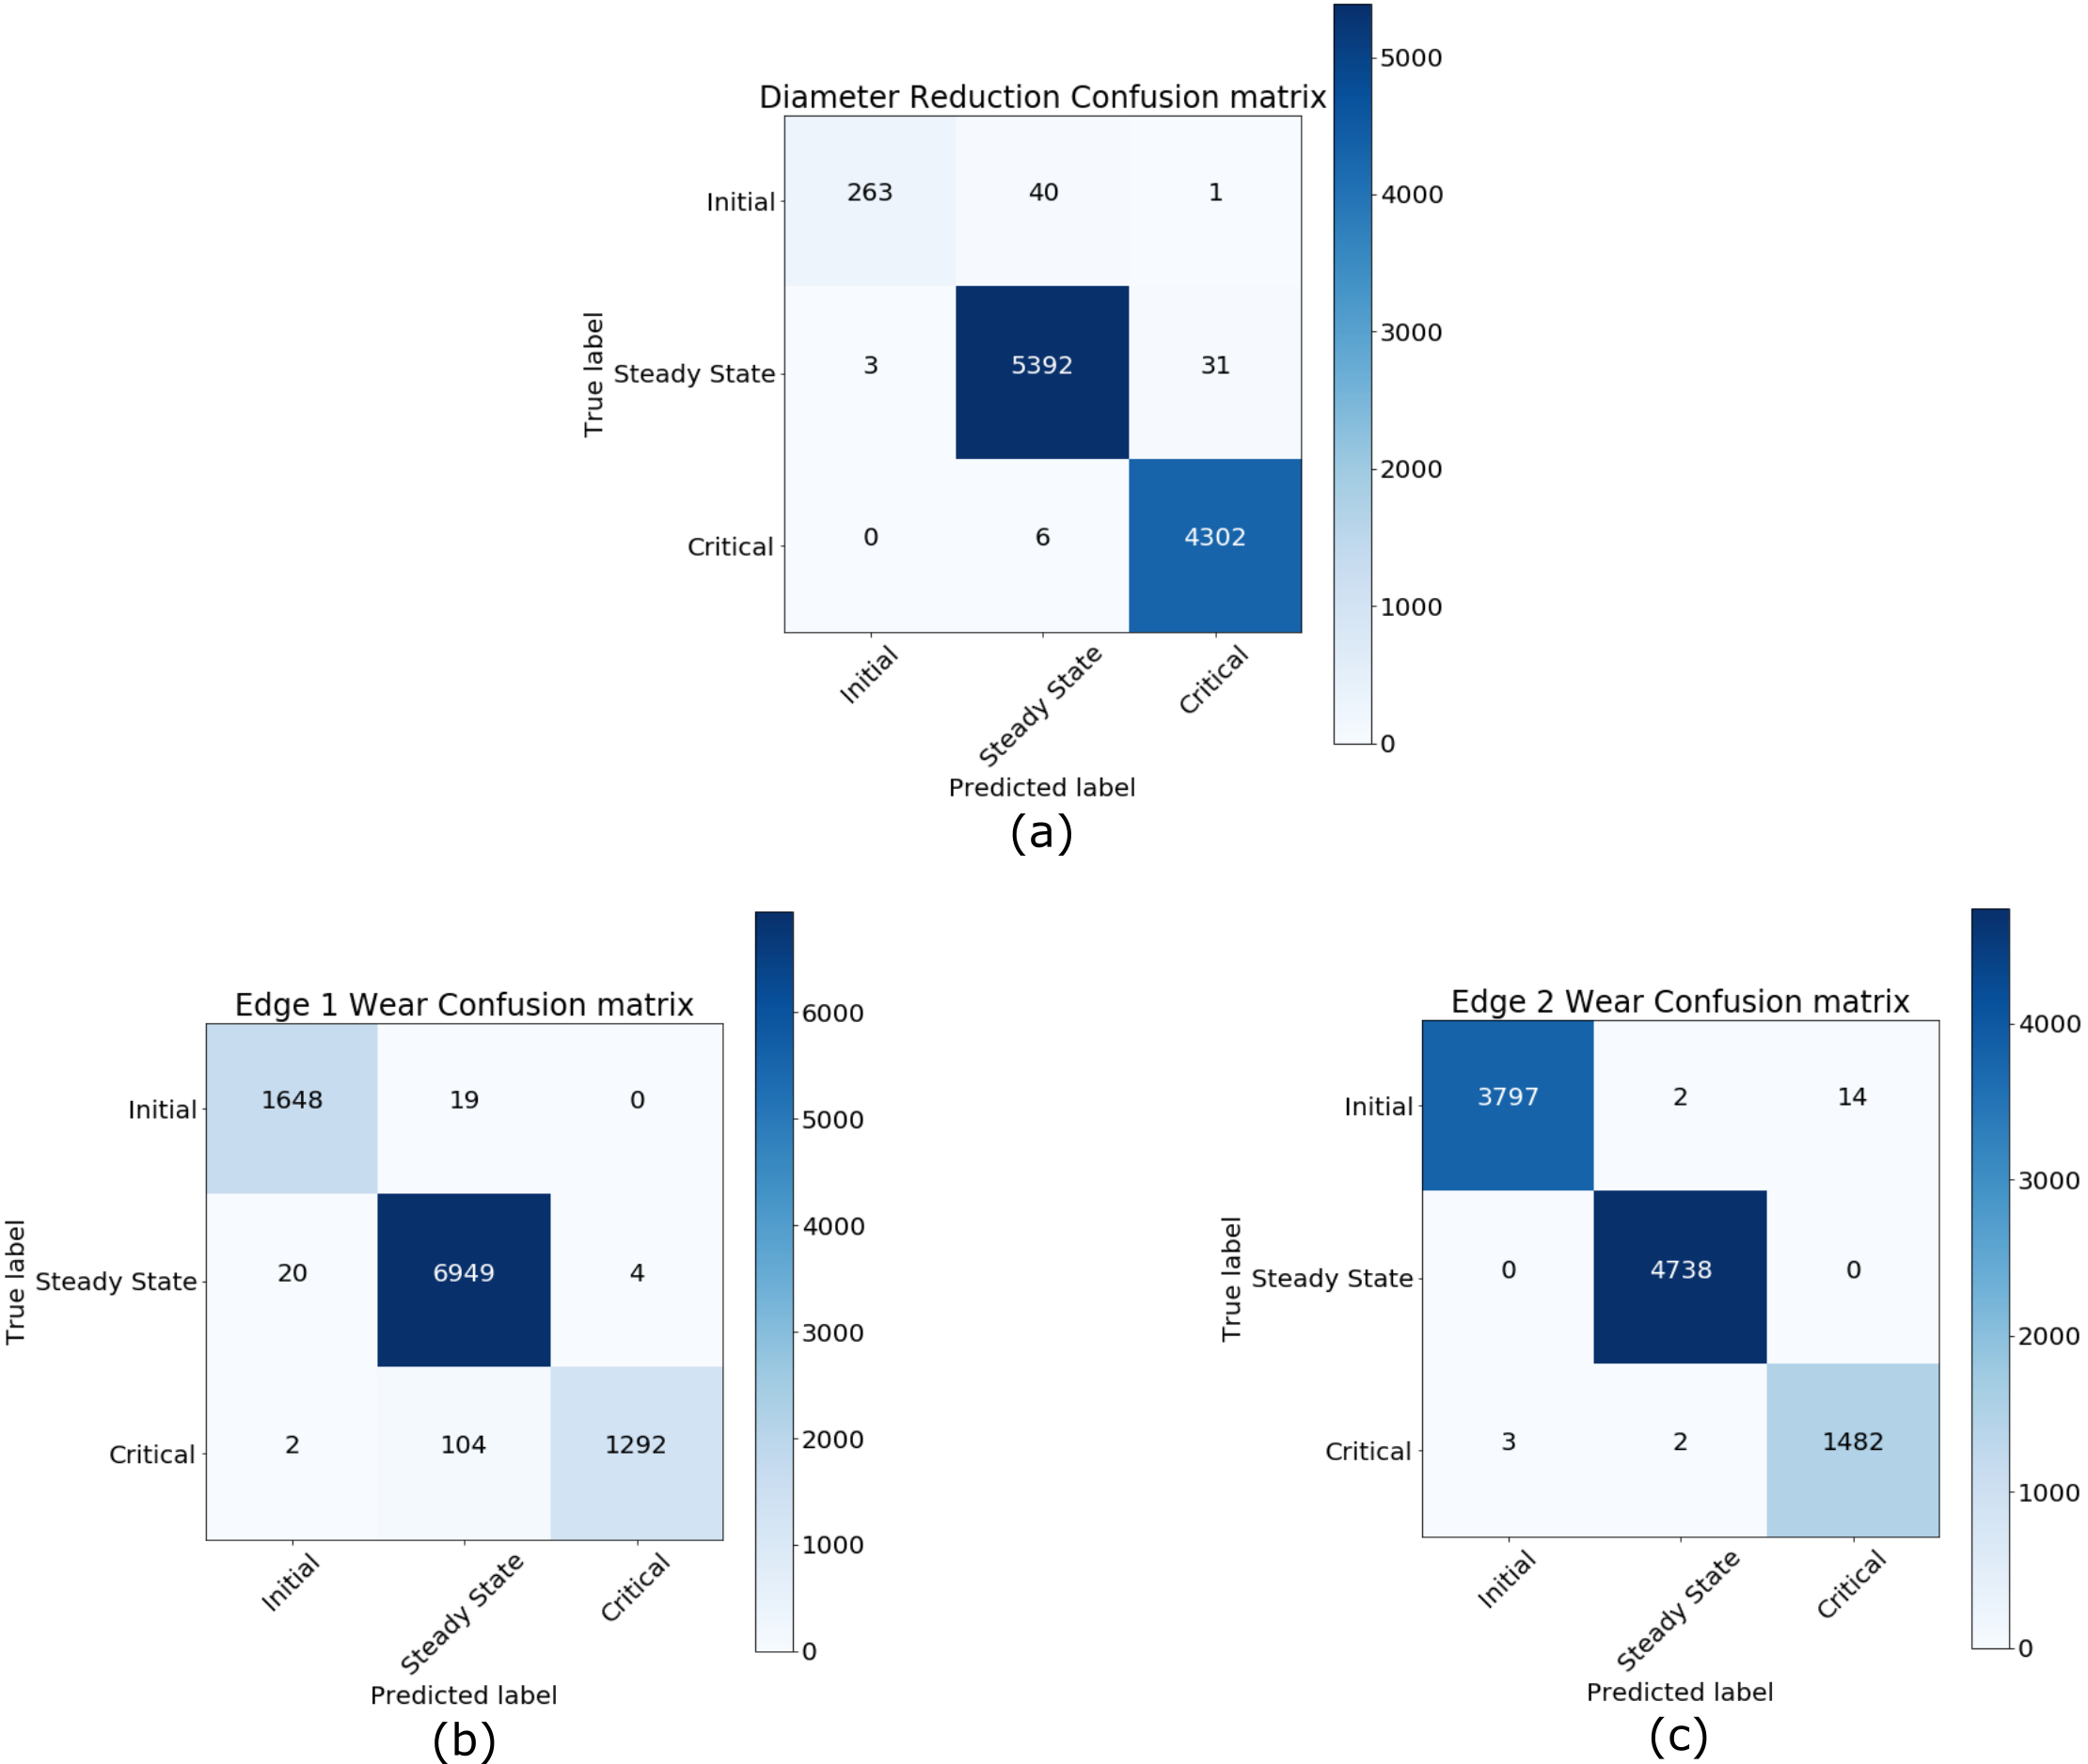
\includegraphics[width=\linewidth]{56.png}
    \caption{ANN Confusion matrices (statistics of true vs predicted labels)}\label{fig:fig56}
  \end{center}
\end{figure}

The trained regression model was tested on each experiment's dataset and the resulting RUL values were predicted. Fig. \ref{fig:fig57} shows the true and predicted RUL values for all the experiments. For T79, T80 and T84 (Fig. \ref{fig:fig57}(a,b,e)), the predicted RUL values at any time instant were underestimated than the actual values. However, for T81, T83 and T86 (Fig. \ref{fig:fig57}(c,d,f)), overestimation in prediction was observed during certain time intervals. \par

\begin{figure}[!h]
  \begin{center}
    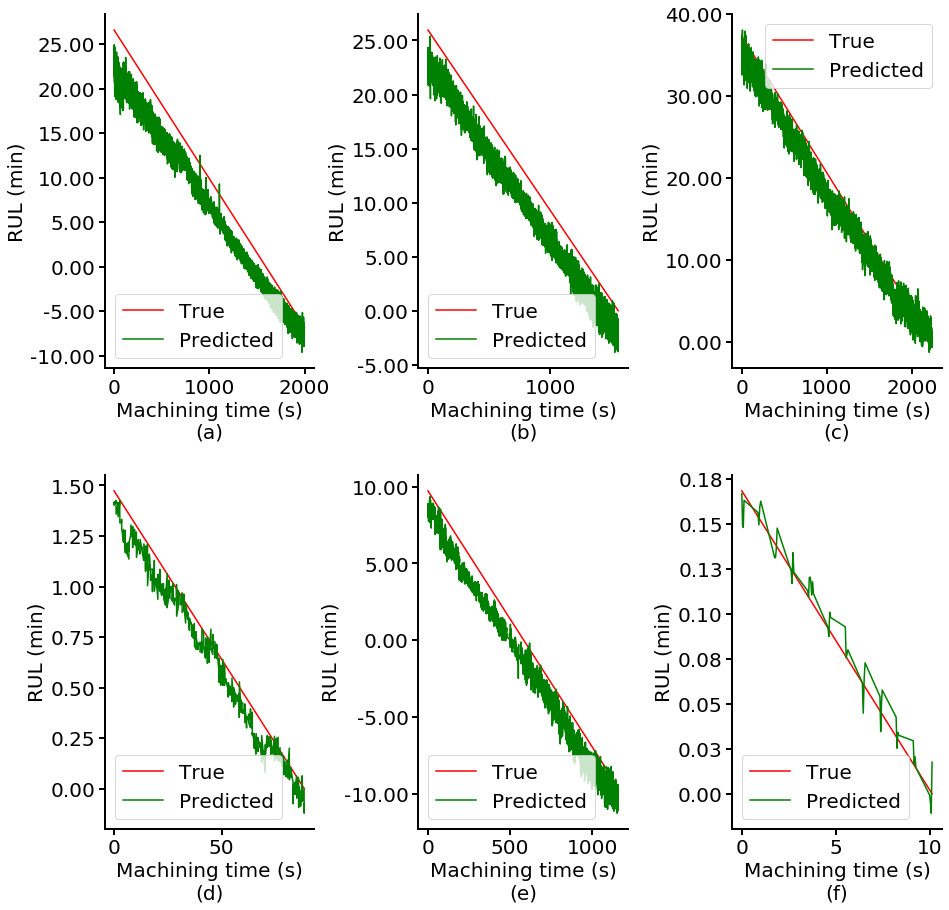
\includegraphics[width=\linewidth]{57.png}
    \caption{ANN RUL predictions}\label{fig:fig57}
  \end{center}
\end{figure}

\subsubsection{DBN performance}
The training of the DBN required a more intesive hyperparameter tuning. The hyperparameters that were taken into account for tuning included the learning rate and number of iterations for the unsupervised pre-training, the learning rate and number of iterations backpropogation, the number of hidden layers and number of neurons per layer.
After training 270 models using different combinations of the hyperparameters mentioned above and cross-validation (RSCV and GSCV), decent performance was obtained for classification with diameter reduction as output. \par

The model performance under four different hyperparameter combinations is shown in Fig. \ref{fig:fig58}. For the training statistics shown in Fig. \ref{fig:fig58}(a,b), the hidden layers structure was kept the same with 2 hidden layers and 63 neurons in each layer along with the other parameters. The backpropogation learning rate of 0.01 (Fig. \ref{fig:fig58}(b)) displayed a \emph{hockey-stick effect} indicating that the learning rate was too small. The \emph{hockey-stick effect} is characterized by a sharp rise or fall of data points after a long flat period and occurs due to poor initialization of the parameters. This effect was not observed when the learning rate was 0.2 (Fig. \ref{fig:fig58}(a)), however, the variability in classification error was too high which indicated a very large learning rate. By keeping the learning rate at 0.05 but increasing the number of hidden layers to 3 (Fig. \ref{fig:fig58}(c)), some improvement was observed in terms of a decrease in the length of the \emph{hockey-stick effect} and the variability. A further improvement was observed when 2 hidden layers were used with 200 neurons in the second hidden layer (Fig. \ref{fig:fig58}(c)). The final structure of the DBN that was used for training is described in Table. \ref{tab:T53} and the classification report from testing data is described in Table. \ref{tab:T54}. \par

\begin{figure}[!h]
  \begin{center}
    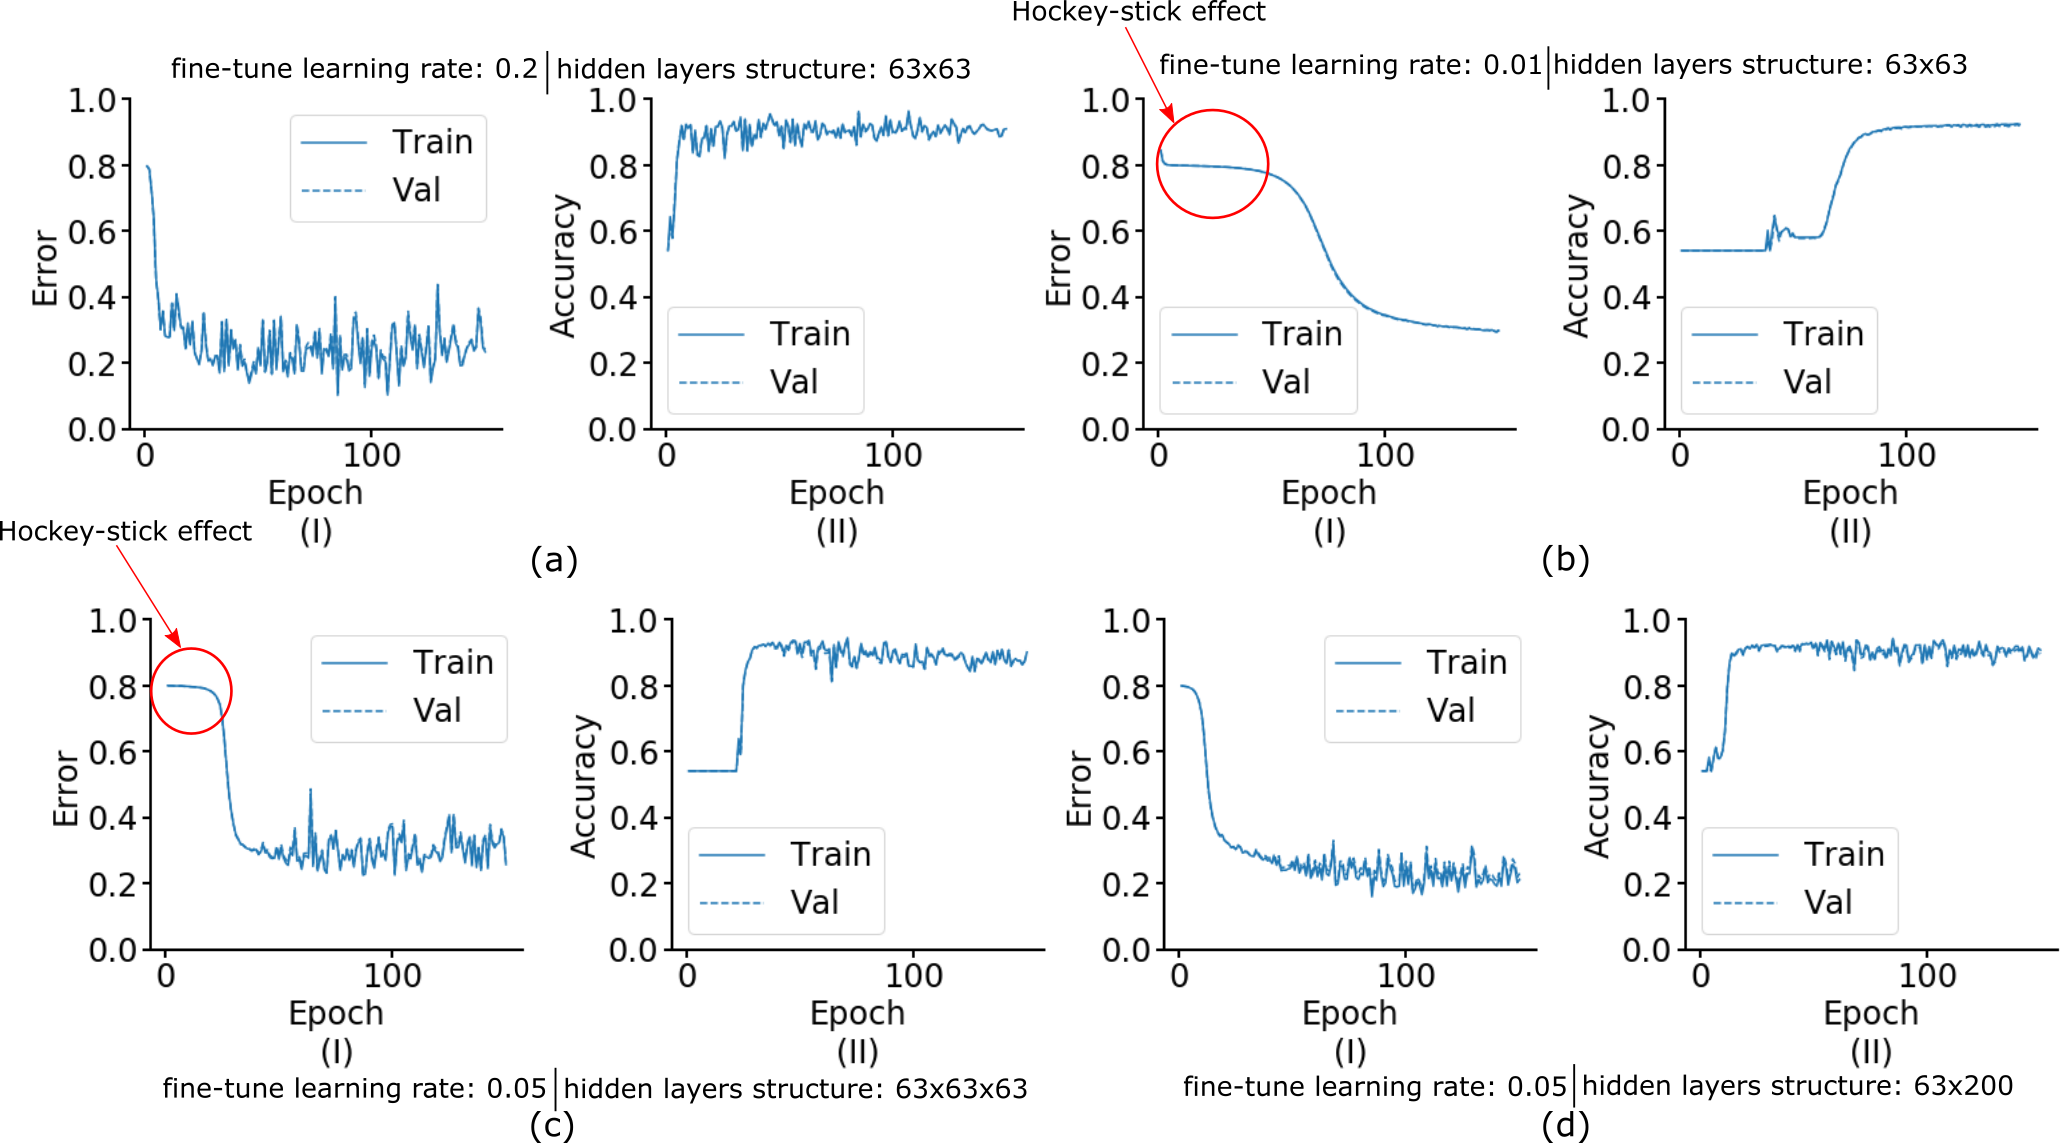
\includegraphics[width=\linewidth]{58.png}
    \caption{DBN hyperparameter tuning (loss and accuracy curves)}\label{fig:fig58}
  \end{center}
\end{figure}

\begin{minipage}{\linewidth}
  \captionof{table}{DBN final architecture details} \label{tab:T53}
  \centering
  \resizebox{0.7\textwidth}{!}{
    \begin{tabular}{ c c c c c c c }
    	\hline
      \makecell{Hidden \\ Layer \\ Structure} & \makecell{RBM learning \\ rate}	& \makecell{Fine-tuning \\ learning rate} & \makecell{RBM \\ epochs} & \makecell{Fine-tuning \\ epochs} & \makecell{Batch Size} & \makecell{Activation \\ function} \\
    	\hline\hline
     	$63$x$200$ & $0.01$ & $0.05$ & $10$ & $150$ & $400$ & $relu$ \\
      \hline
    \end{tabular}}
\end{minipage} \\\\

\begin{minipage}{\linewidth}
  \captionof{table}{DBN testing statistics for diameter reduction based classification} \label{tab:T54}
  \centering
  \resizebox{0.6\textwidth}{!}{
    \begin{tabular}{c | c c c c }
    	\hline
      \makecell{Class} & \makecell{Precision} & \makecell{Recall}	& \makecell{F1-score} & \makecell{Support} \\
    	\hline\hline
     	Initial Wear & $0.87$ & $0.26$ & $0.4$ & $304$ \\
      \hline
      Steady State Wear & $0.91$ & $0.95$ & $0.93$ & $5426$ \\
      \hline
      Critical Wear & $0.93$ & $0.93$ & $0.93$ & $4308$ \\
      \hline\hline
      Accuracy & $-$ & $-$ & $0.92$ & $10038$ \\
      \hline
      Macro Average & $0.9$ & $0.71$ & $0.75$ & $10038$ \\
      \hline
      Weighted Average & $0.92$ & $0.92$ & $0.91$ & $10038$ \\
      \hline
    \end{tabular}}
\end{minipage} \\\\

The relatively lower accuracy of DBN(93\%), compared to the ANN(98\%), indicates the possibility that the set of hyperparameters used may not be ideal. As can be seen from Fig. \ref{fig:fig58}(d), some amount of variability is still present in the model with the chosen set of hyperparameters (Table. \ref{tab:T53}). In order to obtain a smooth convergence of error with no \emph{hockey-stick effect}, a significantly larger number of different hyperparameter combinations need to be used to train and evaluate an equal number of models. This process demands higher computational power to achieve reasonable training times which was unavailable during this research. Also, the high value of precision but a drastically lower recall for the initial wear region indicates that the model is able to distinguish this state from the other states correctly but is unable to accurately predict it (find the boundary between initial wear and steady state wear). This is primarily because of the relatively lower support-value for this class and suggests that tool wear sampling in the initial phases (first 200 slots) of the experiment be done at a higher frequency to obtain the exact differential in tool condition. \par

\iffalse
\subsubsection{Importance of TPR in prediction (SHAP values)}

The impact of tool path radius, and other features, on the prediction of tool wear state and remaining-useful-life was also studied using SHAP (SHapley Additive exPlanations) values \cite{CITE34}. SHAP values break down a prediction to show the impact of each feature. The goal of SHAP is to explain the prediction of an instance x by computing the contribution of each feature to the prediction. The SHAP feature importance is based on the idea that features with large absolute Shapely values are important. The global importance is then calculated based on the average of the absolute Shapely values per feature across the data.\par

The SHAP values for the input feature array in the testing dataset were calculated using a Deep Explainer estimator (readers are referred to the SHAP documentation for detailed explanation). A summary plot of the feature importance on the input feature array (63 features) was then generated for each output label (Fig. \ref{fig:fig59}). The most important feature for wear state classification was found to be the $fz\_mean$. However the static radial tool runout was of significant importance too. This confirms the previous observations about the impact of static runout on the premature tool failure. \par

\begin{figure}[!h]
  \begin{center}
    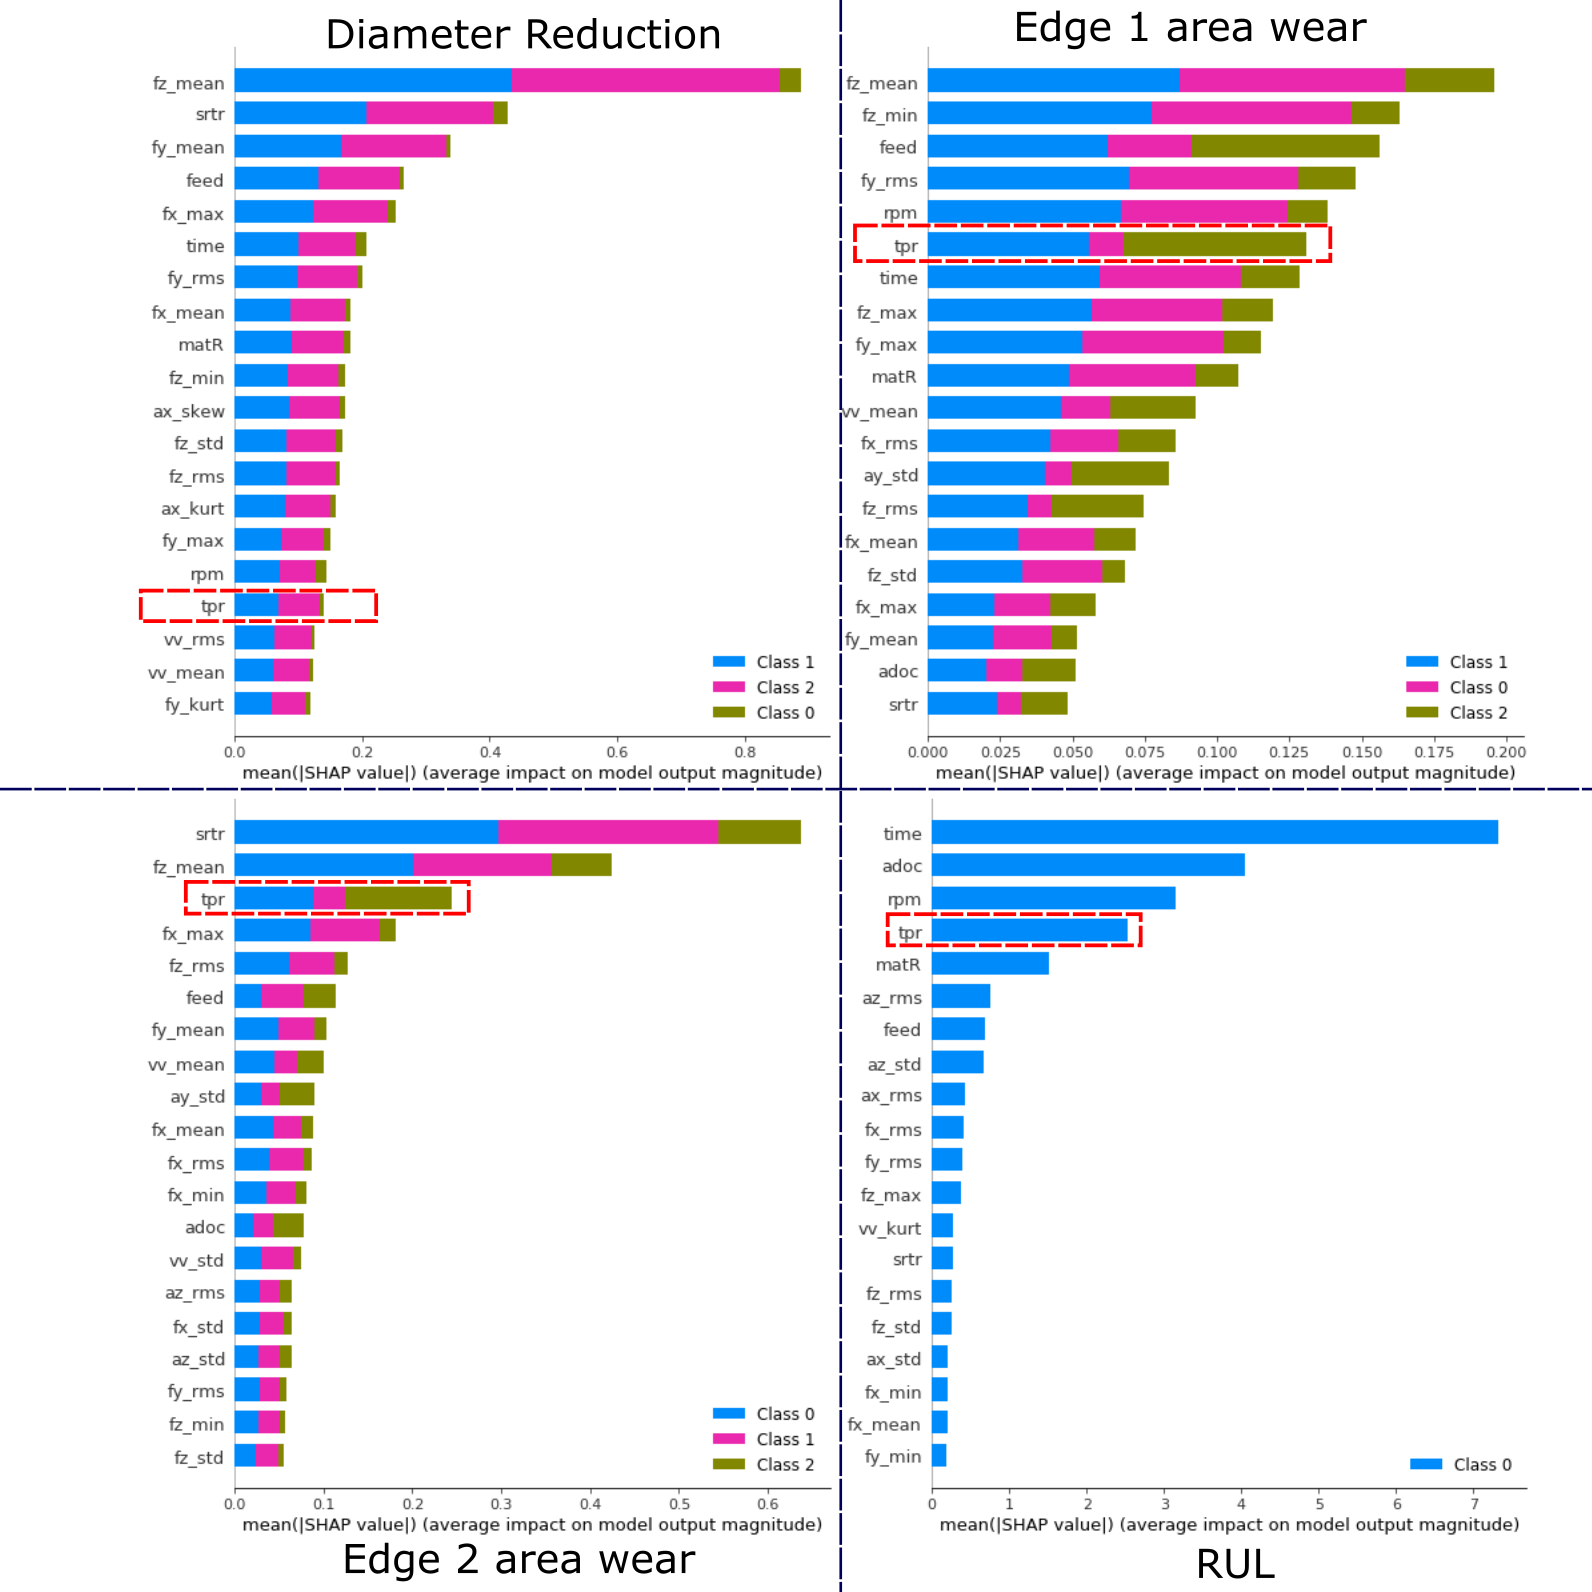
\includegraphics[width=\linewidth]{59.png}
    \caption{Summary plots indicating feature importance using SHAP values}\label{fig:fig59}
  \end{center}
\end{figure}

However, the important observation, relevant to the main aim of this study, was the quantification of the impact of tool path radius on wear state classification and RUL predictions. It can seen that the tool path radius (tpr), on an average, changes the predicted wear state by 1-2\% and is amongst the top 20 features (out of the 63 features) in affecting the outcome. This clearly shows that tool path radius, as a process parameter, is of significant importance in the classification of wear state as well as RUL.
\fi

%==========================================================================================================%
%\iffalse
\section{Conclusions}\label{chap:conc}

This paper investigated the impact of tool path radius on cutting tool wear in micro end-milling processes. A unique set of experiments involving semi-circular tool paths, varying spindle speed and feed was designed. The process of generating g-codes for the machining the slots in different batch sizes was automated. Cutting data was generated from sensors in the form of force, acceleration and vibration velocity. The static radial tool runout and intermediate images of the tool face were captured to generate tool wear data. Sensor data was segmented to isolate individual slot data using k-means clustering and peaks-analysis algorithms. Subsequently, various statistical features were extracted by grouping the sensor data of each slot into 4 segments which generated a total of 33460 data points. \par

The denoised, coloured tool images were binarized and aligned with respect to base image. The final image for measuring the wear features was obtained by taking a difference between the binarized intermediate tool image and the binarized base image. The extracted features from the final image included the chipped area of individual cutting edges and diameter reduction values. Tool state was classified into three regions based on diameter reduction and chipped area of individual cutting edges by defining specific criteria for each. The remaining-useful-life for a particular data point was calculated by taking the difference between the first time instant when the tool reached the end-of-tool-life criteria and the time instant of that data point. \par

The progression of tool wear was modelled using artificial neural network (ANN) and deep belief network (DBN) to capture the non-linear relation of tool path radius along with the other process parameters and sensor data. For classification with ANN, single hidden layer with 63 neurons were used while two hidden layers with 63 and 200 neurons each were used for DBN. Regression analysis for predicting RUL was done using ANN with two hidden layers with 63 and 200 neurons each. Adam optimizer was used for training ANN to improve rate of convergence of prediction error. The DBN training involved an unsupervised pre-training using 10 iterations for initializing the weights and the biases. This was followed by a supervised fine-tuning of the weights and biases using stochastic gradient descent technique. \par

The training performance of the model was improved using hyperparameter tuning techniques. Hyperparameters that were tuned included the learning rate, number of training iterations and hidden layers structure. This involved training models with 270 different hyperparameter combinations and the one with the best performance during training was selected. The final, trained models where then evaluated on the testing dataset to evaluate their performance. The following were the main conclusions drawn from this study. \par

\begin{itemize}
  \item In the case where the tool broke, a significant rise in peak-to-peak, z-direction forces was observed. Similar force signatures were observed when tool reached end-of-life. Such force signatures can be used as indicators of nearing the end-of-tool-life or potential breakage.
  \item Wear rates for higher tool path radius (500 $\mu{m}$) were significantly higher than lower tool path radius (250 $\mu{m}$). For tpr of 750 $\mu{m}$, sudden, catastrophic tool failure was observed after machining only 10-15 slots.
  \item Lower tpr showed edge rounding and significant flank wear of the tool before breakage. However for 500 $\mu{m}$ tpr, adhesive wear was found to be the major wear mechanism along with edge rounding and flank wear. For higher tpr, severe chipping along with adhesive wear lead to catastrophic tool failure.
  \item The monitoring of individual edge wear revealed the switch in active cutting edges while machining. In some cases, there was a switch in active cutting edge just before tool breakage. Such a monitoring strategy could provide more reliable information about tool condition and thus enable better decision making during on-line machining.
  \item The wear state classification accuracy, for ANN model, with invidual edge wear as output label was found to be higher (99\%) than with diameter reduction as output label (98\%). This indicates that monitoring the wear progression of indvidual cutting edges could provide better prognostics insights.
  \item Regression analysis for tool remaining-useful-life indicated both underestimation and overestimation in predictions with a cosine-value of 0.96. However, the degree by which the results were underestimated was much higher than the overestimated results indicating an overall conservative prediction nature.
  \item The testing of deep belief networks revealed a slight degradation in classification of wear state (93\% accuracy) as compared to the backpropogated artificial neural networks (98\% accuracy). This could be significantly improved by implementing a more rigourous and dense hyperparameter tuning technique.
\end{itemize}




\iffalse
\item Feature importance analysis for model prediction shows that tool path radius has significant weightage in driving the wear state classification as well as RUL prediction. This result reinforces the need the include such a process parameter for a more accurate tool condition monitoring in micro end-milling processes.

The incorporation of a novel process parameter for micro milling processes, representing non-linearity of tool paths, has revealed that the wear progression of micro-tools can be altered significantly by controlling this parameter. Every complex curve with varying radii of curvature (ROC) can effectively be described as a combination differential curves having constant ROC.
\fi

%\fi

%% The Appendices part is started with the command \appendix;
%% appendix sections are then done as normal sections
%% \appendix

%% \section{}
%% \label{}

%% References
%%
%% Following citation commands can be used in the body text:
%% Usage of \cite is as follows:
%%   \cite{key}          ==>>  [#]
%%   \cite[chap. 2]{key} ==>>  [#, chap. 2]
%%   \citet{key}         ==>>  Author [#]

%% References with bibTeX database:
\newpage
\bibliographystyle{unsrt}
\nocite{*}
\bibliography{cite_p.bib}
%\printbibliography

%% Authors are advised to submit their bibtex database files. They are
%% requested to list a bibtex style file in the manuscript if they do
%% not want to use model1-num-names.bst.

%% References without bibTeX database:

% \begin{thebibliography}{00}

%% \bibitem must have the following form:
%%   \bibitem{key}...
%%

% \bibitem{}

% \end{thebibliography}


\end{document}

%%
%% End of file `elsarticle-template-1-num.tex'.
